\documentclass[9pt,journal,compsoc]{IEEEtran}
\usepackage{amsmath,amssymb,amsbsy}
\usepackage{graphicx}
\usepackage{balance}  % for  \balance command ON LAST PAGE  (only there!)
\usepackage{url}
\usepackage{enumitem}
\usepackage{hyperref}
\usepackage{multirow}
\usepackage{gensymb}
\usepackage{subcaption}
\usepackage[export]{adjustbox}
\usepackage{tabularx, colortbl}
\usepackage{array}
\usepackage{dblfloatfix}
\usepackage{fancyvrb}
\usepackage{gensymb}
\usepackage{listings}
\usepackage{color,soul}
\usepackage{courier}

\definecolor{codegreen}{rgb}{0,0.6,0}
\definecolor{codegray}{rgb}{0.5,0.5,0.5}
\definecolor{codepurple}{rgb}{0.58,0,0.82}
\definecolor{co_string}{RGB}{95, 135, 0}
\definecolor{co_comment}{RGB}{135, 135, 135}
\definecolor{co_other}{RGB}{135, 95, 175}
\definecolor{co_number}{RGB}{215, 95, 0}
\definecolor{co_keyword}{RGB}{215, 0, 95}
\definecolor{co_special}{RGB}{0, 135, 175}

\lstdefinestyle{custompy}{
    basicstyle=\footnotesize\ttfamily,
    commentstyle=\color{co_comment},
    keywordstyle=\bfseries\color{co_keyword},
    keywordstyle=[2]{\bfseries\color{co_other}},
    stringstyle=\bfseries\color{co_string},
    emphstyle=\bfseries\color{co_special},
    breakatwhitespace=false,
    breaklines=true,
    captionpos=b,
    keepspaces=true,
    showspaces=false,
    showstringspaces=false,
    showtabs=false,
    tabsize=2,
    literate=%
        {0}{{{\color{co_number}0}}}1
        {1}{{{\color{co_number}1}}}1
        {2}{{{\color{co_number}2}}}1
        {3}{{{\color{co_number}3}}}1
        {4}{{{\color{co_number}4}}}1
        {5}{{{\color{co_number}5}}}1
        {6}{{{\color{co_number}6}}}1
        {7}{{{\color{co_number}7}}}1
        {8}{{{\color{co_number}8}}}1
        {9}{{{\color{co_number}9}}}1,
}

\begin{document}
\bstctlcite{IEEEexample:BSTcontrol}

\title{Synopsis: A Distributed Sketch over Voluminous Spatiotemporal Observational Streams}

\author{Thilina~Buddhika, Matthew Malensek, Sangmi Lee Pallickara and Shrideep Pallickara,~\IEEEmembership{Members,~IEEE}%
%\IEEEcompsocitemizethanks{\IEEEcompsocthanksitem T. Buddhika, M. Malensek, S.L. Pallickara and S. Pallickara  are with the Department
%of Computer Science, Colorado State University.
%E-mail: \{thilinab, malensek, sangmi, shrideep\}@cs.colostate.edu\protect}
}

\IEEEtitleabstractindextext{%
\begin{abstract}
    Networked observational devices have proliferated in recent years, contributing to voluminous data streams from a variety of sources and problem domains. These streams often have a spatiotemporal component and include multidimensional \emph{features} of interest. Processing such data in an offline fashion using batch systems or data warehouses is costly from both a storage and computational standpoint, and in many situations the insights derived from the data streams are useful only if they are timely.

    In this study, we propose \textsc{Synopsis}, an online, distributed \emph{sketch} that is constructed from voluminous spatiotemporal data streams. The sketch summarizes feature values and inter-feature relationships in memory to facilitate real-time query evaluations and to serve as input to computations expressed using analytical engines. As the data streams evolve, \textsc{Synopsis} performs targeted dynamic scaling to ensure high accuracy and effective resource utilization. We evaluate our system in the context of two real-world spatiotemporal datasets and demonstrate its efficacy in both scalability and query evaluations.
\end{abstract}
\begin{IEEEkeywords}
data sketches, streaming systems, spatiotemporal data, query evaluations
\end{IEEEkeywords}}
\maketitle

\IEEEdisplaynontitleabstractindextext
%
% Introduction
%
\section{Introduction}
\label{sec:introduction}
The proliferation of remote sensing equipment such as radars and satellites, networked sensors, commercial mapping, location-based services, and sales tracking applications have resulted in exponential growth of spatiotemporal data. Such datasets comprise observations where both the location and time of measurement are available in addition to \emph{features} of interest (such as humidity, air quality, disease prevalence, sales, etc.). This information can be leveraged in several domains, including atmospheric science, epidemiology, environmental science, geosciences, smart cities, and commercial applications. In these settings, queries over the data must be \emph{expressive} and execute in real time, regardless of data volumes.

Spatiotemporal datasets are naturally multidimensional with multiple features of interest being reported/recorded continuously for a particular timestamp and geolocation. The values associated with these features are continually changing; in other words, the dataset \emph{feature space} is always evolving.  Queries specified over these datasets may have a wide range of characteristics encompassing the frequency at which they are evaluated and their spatiotemporal scope. The crux of this paper is to support query evaluations and data processing over continually-arriving observational data. We achieve this via construction of an in-memory distributed \emph{sketch} that maintains a compact representation of the data.
The sketch is also an effective surrogate for the data that it snapshots and serves as input for computations.
%
%
\vspace{1.7em}\\
%
\textbf{Challenges:} \hl{Support for real-time evaluation of queries and analysis over a feature space that is continually evolving introduces unique challenges. These include:}
\begin{itemize}[leftmargin=*]
    \item   \emph{Data volumes and arrival rates:} It is infeasible to store all observations, which may arrive continually and at high rates. This is especially true if the arrival rates outpace disk speeds.
    \item \emph{I/O Costs:} Memory accesses are 5-6 orders of magnitude faster than disk accesses. Given the data volumes, disk accesses during query evaluations or analysis are infeasible.
    \item   \emph{Accuracy:} Queries evaluations must be accurate, with appropriate error bounds included in the results.
    \item   \emph{Spatiotemporal characteristics:} Queries and analysis may target both spatial and chronological properties of the dataset.
\end{itemize}
%
\vspace{0.7em}
%
\textbf{Research Questions:} \hl{The challenges associated with accomplishing this functionality led us to formulate the following:}
\begin{description}[leftmargin=*]
    \item[\emph{RQ-1:}] How can we generate compact, memory-resident representations of the observational space while accounting for spatiotemporal attributes? The resulting \emph{sketch} must be amenable to fast, continuous updates to ensure its representativeness and fidelity to the original data.
    \item[\emph{RQ-2:}] How can we scale effectively in situations where system load is high or observations arrive faster than the sketch can be updated? The density and arrival rates for observations may vary based on geospatial characteristics; for example, New York would have a far higher rate of observations than Denver.
    \item[\emph{RQ-3:}] How can we enable expressive, low-latency queries over the distributed sketch while also maintaining accuracy?  Given that the sketch is a compact representation of the data, queries facilitate high-level analysis without requiring users to understand the underlying system implementation.
\end{description}
%
\vspace{0.7em}
%
\textbf{Approach Summary}:
Similar to other sketches, the design of \textsc{Synopsis} was guided by its desired functionality. \textsc{Synopsis} is a compact, effective surrogate for voluminous data; the system extracts metadata from observations and organizes this information to support relational queries targeting different portions of the feature space. We support selection, joins, aggregations, and sorting. The \textsc{Synopsis} sketch can interoperate and provide input data to general purpose computations expressed using popular analytic engines such as Spark \cite{zaharia2010spark,armbrust2015spark}, TensorFlow \cite{abadi2016tensorflow,tensorflow}, Hadoop \cite{hadoop,shvachko2010hadoop,borthakur2008hdfs}, and VW \cite{langford2007vowpal}.

Our sketch is also naturally amenable to distribution, with each machine in the cluster holding information about a particular subset of the observational space.  This ensures that each cluster-node can evaluate multiple concurrent queries independently. The sketch is capable of scaling in or out depending on streaming ingress rates and memory footprints, with scale-out operations that support targeted alleviation of hotspots. \textsc{Synopsis} manages the complexity of identifying these hotspots, splitting portions of the sketch, and migrating relevant subsets. Distributing the sketch allows us to maintain a finer-grained representation of the feature space while also improving the accuracy of query evaluations; e.g., an arctic region and a tropical region would be maintained on separate nodes that specialize for particular climates.
%
\vspace{0.7em}\\
%
\textbf{Paper Contributions}:
To our knowledge, \textsc{Synopsis} is the first sketch tailored specifically for spatiotemporal observational data. The methodology of this study is centered around our novel in-memory data structure, \emph{SIFT} (\S\ref{sec:sift}), which employs a hierarchical forest-of-trees approach combined with online, running summary statistics to compactly represent observational data. In addition to the memory benefits of the SIFT, the data structure is amenable to distribution across a cluster of machines. This allows \textsc{Synopsis} to cope with high-rate data arrivals and scale dynamically with changes in problem size or resource availability. Both dynamic scaling and querying are facilitated by efficient tree-based lookup operations. For analytic tasks, the SIFT acts as an effective surrogate for full-resolution observations, enabling expressive queries over arbitrary spatiotemporal scopes, generation of synthetic datasets, and interoperation with popular analytical engines.
%
\vspace{0.7em}\\
%
\textbf{Paper Organization}:
\S\ref{sec:system} provides a system overview, followed by methodology in \S\ref{sec:methodology}. A performance evaluation is presented in \S\ref{sec:performance}, while \S\ref{sec:applications} demonstrates applications of \textsc{Synopsis}, \S\ref{sec:related} discusses related approaches, and \S\ref{sec:conclusions} concludes the paper.
\vspace{-0.7em}
%
% System Overview
%
\section{System Overview and Preliminaries}
\label{sec:system}
\textsc{Synopsis} is a distributed sketch constructed over voluminous spatiotemporal data streams.
The number of sketchlets (executing on different machines) that comprise the distributed sketch varies dynamically as the system scales in or out to cope with data arrival rates and memory pressure.
%Each sketchlet is responsible for one or more geographical scopes and is implemented as a stateful stream processing node that can build and retain state over time.
\textsc{Synopsis} assimilates, organizes, and compacts spatiotemporal data streams that comprise the sketch.
A stream partitioning scheme, based on the Geohash algorithm, is used to route packets to the appropriate sketchlet.
Sketchlets process stream packets emitted by stream ingesters and construct compact, in-memory representations of the observational data by extracting metadata from stream packets.
During dynamic scaling, the geographic extents managed by a sketchlet vary.
%
\vspace{0.7em}\\
%
\textbf{System Components}:
\textsc{Synopsis} \hl{leverages the Neptune stream processing system}~\cite{buddhika2016neptune, buddhika2017online} and relies on a set of auxiliary services that are needed to construct, update, and maintain the sketch, as well as adapt to changing system conditions:
\begin{description}[leftmargin=*]
\item[Control plane] is responsible for orchestrating control messages exchanged between sketchlets as part of various distributed protocols such as dynamic scaling.
    It is decoupled from the generic data plane to ensure higher priority and low latency processing without being affected by buffering delays and backpressure experienced during stream processing.

\item[Gossip subsystem] is used by the sketchlets to gossip about their state periodically (based on time intervals and the number of pending updates) as well as when a change in state occurs to establish an approximate global view of the system. \textsc{Synopsis} supports \emph{eventual consistency} with respect to these updates given their propagation and convergence delays.

\item[Querying subsystem] is responsible for the distributed evaluation of queries.
    This involves forwarding queries to relevant sketchlets; in some cases, multiple sketchlets may be involved based on the geographical scope of the query.

\item[Monitoring subsystem] probes sketchlets comprising \textsc{Synopsis} periodically to gather metrics that impact performance of the system.
    These include memory utilization and backlog information based on packet arrival rates and updates to the in-memory structures.
    This information is used for dynamic scaling recommendations as explained in Sections~\ref{subsec:scaling-out} and \ref{subsec:scaling-in}.
\end{description}
%
\textbf{Data Model}:
While designing \textsc{Synopsis}, we targeted a data model wherein observations are geotagged and have chronological timestamps indicating where and when the observations were made. Location information is encoded as $\langle latitude, longitude \rangle$ tuples. Observations contain multiple features (temperature, humidity, wind speed, etc.), and may be encoded as $\langle feature\_name, value \rangle$ tuples or may have predefined positions within the serialized data representation. 
%
\vspace{0.7em}\\
%
\textbf{Query Support}:
\textsc{Synopsis} supports common query constructs such as selects or joins, while also providing rich analytical queries that report statistical information, make predictions, or produce synthetic datasets (detailed fully in \S\ref{subsec:query-eval}). A key innovation in our query support is that portions of the sketch itself can be retrieved and manipulated by clients. The following query demonstrates this functionality, where climate features are requested from a region when the wind speed is more than a standard deviation away from the mean:

\begin{lstlisting}[language=SQL,style=custompy]
   SELECT location, precipitation, humidity
   WHERE location LIKE 'dj%' AND
       (wind_sp > MEAN(wind_sp) + STD(wind_sp)
       OR wind_sp < MEAN(wind_sp) - STD(wind_sp))
\end{lstlisting}
%
%\vspace{0.7em}\\
%
\textbf{Stream Partitioning}:
We use the Geohash~algorithm~\cite{geohash} to balance load and partition incoming data streams. Geohash divides the earth into a hierarchy of bounding boxes identified by Base 32 strings; the longer the geohash string, the more precise the bounding box. Figure~\ref{fig:geohash} illustrates this hierarchy. Most of the eastern United States is contained within the bounding box described by geohash \emph{D}, while \emph{DJ} encompasses substantial parts of Florida, Georgia, and Alabama. The bounding box \emph{DJKJ} (highlighted in red) contains Tallahassee, Florida. This hierarchical representation enables \textsc{Synopsis} to cope with both low- and high-density regions: several sketchlets may be tasked with managing streams originating in and around large cities, while rural areas fall under the purview of a single node.

Each bit added to a geohash string reduces its scope by half, with each character represented by five bits ($2^5 = 32$). In other words, a four-character geohash string represents 20 spatial subdivisions applied recursively to each resulting region. This property allows us to manage and allocate resources across a variety of observational densities.

\begin{figure}[h!]
    \centerline{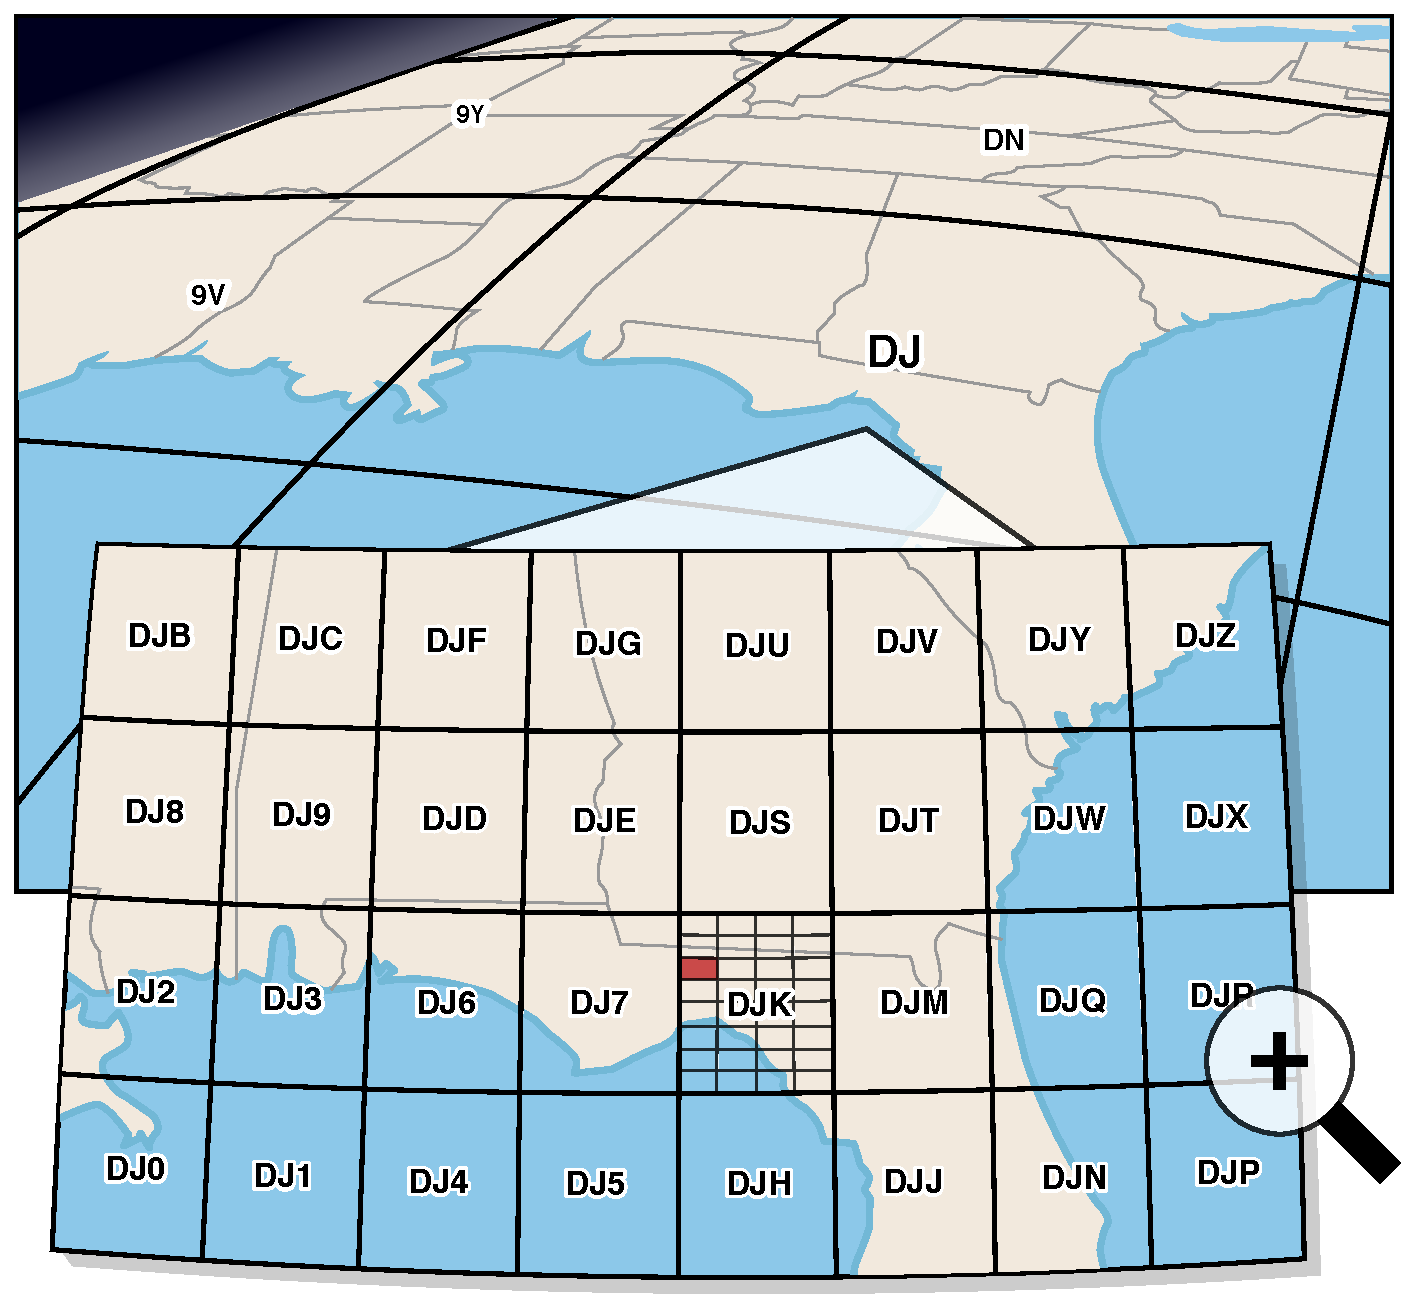
\includegraphics[width=2.5in]{figures/geohash.pdf}}
    \caption{Visual demonstration of the Geohash algorithm.}
    \label{fig:geohash}
\end{figure}
%
% Methodology
%
\section{Methodology}
\label{sec:methodology}
In this section, we discuss the construction of the distributed sketch, sketchlet data structure, dynamic scaling, and query support in \textsc{Synopsis}. We report microbenchmark results which were run using a single machine (HP DL160; Xeon E5620; 12 GB RAM) demonstrating the efficacy of individual aspects of the system. Our input data was sourced from NOAA North American Mesoscale (NAM) Forecast System \cite{noaa_nam}.

\subsection{Sketch}
From a macroscopic view, the sketch is organized as a distributed prefix tree. All descendant nodes -- \emph{sketchlets} -- are responsible for a particular geospatial scope and share a common prefix with their parent. One of our primary goals behind \textsc{Synopsis} is to ensure the sketch is performant, flexible, and amenable to scaling. The sketch initiates scale-out operations to relieve memory pressure and preserve performance, while scale-in operations conserve memory. Further, any sketchlet may serve as the \emph{conduit} for queries or analytic operations.

The geohash algorithm plays a central role in the organization of the distributed sketch. Since locations are represented by bounding boxes, the algorithm facilitates collocation of observations from particular geographical scopes. This allows the conduit to redirect queries effectively and ensure data locality. Increases in the length of the geohash string correspond to geographically smaller (and more precise) bounding boxes. This is well-aligned with dynamic scaling performed by the sketch to manage memory requirements. Scaling operations within the sketch are targeted; scaling out targets geospatial locations with increased density of observations to relieve memory pressure and alleviate performance bottlenecks, while scaling in targets geolocations where there is a sparsity in available data to conserve memory.

Each sketchlet is responsible for real-time organization, summarization, and compaction of observational data from the geographical scope represented by its geohash. The sketchlet performs two operations: first, it extracts metadata from incoming observations, including geolocations, chronological information, and features encapsulated within the observation. Second, the sketchlet is responsible for summarization and compaction of the extracted features.

The sketchlet organizes its summarization in a data structure called SIFT (Summarization Involving a Forest of Trees). The edges and vertices within each SIFT tree maintain inter-feature relationships, while leaves contain online, in-memory summary statistics and correlation information to support statistical queries and generation of synthetic datasets.  The number of edges at each level within the subtrees corresponds to density-based dynamic binning of a particular feature to reduce error. The underlying principle within this data structure is \textbf{grouping} to exploit similarities in values reported within observations; grouping allows us to preserve fidelity of the observational space while conserving memory.

A simplified version of the distributed sketch for geospatial region \emph{D} is depicted in Figure~\ref{fig:dist-sketch}. Each tree within the SIFT is rooted at a higher precision geohash than that associated with the sketchlet. For example, at a sketchlet with a geohash prefix, \emph{DJ}, the trees within the SIFT at that sketchlet are rooted at higher precision geohashes such as \emph{DJB}, \emph{DJC}, \emph{DJF}, etc. An advantage of this approach is that the sketchlet partitions data from the overall geospatial scope into smaller regions, further improving the grouping of observations.

\begin{figure}
    \centerline{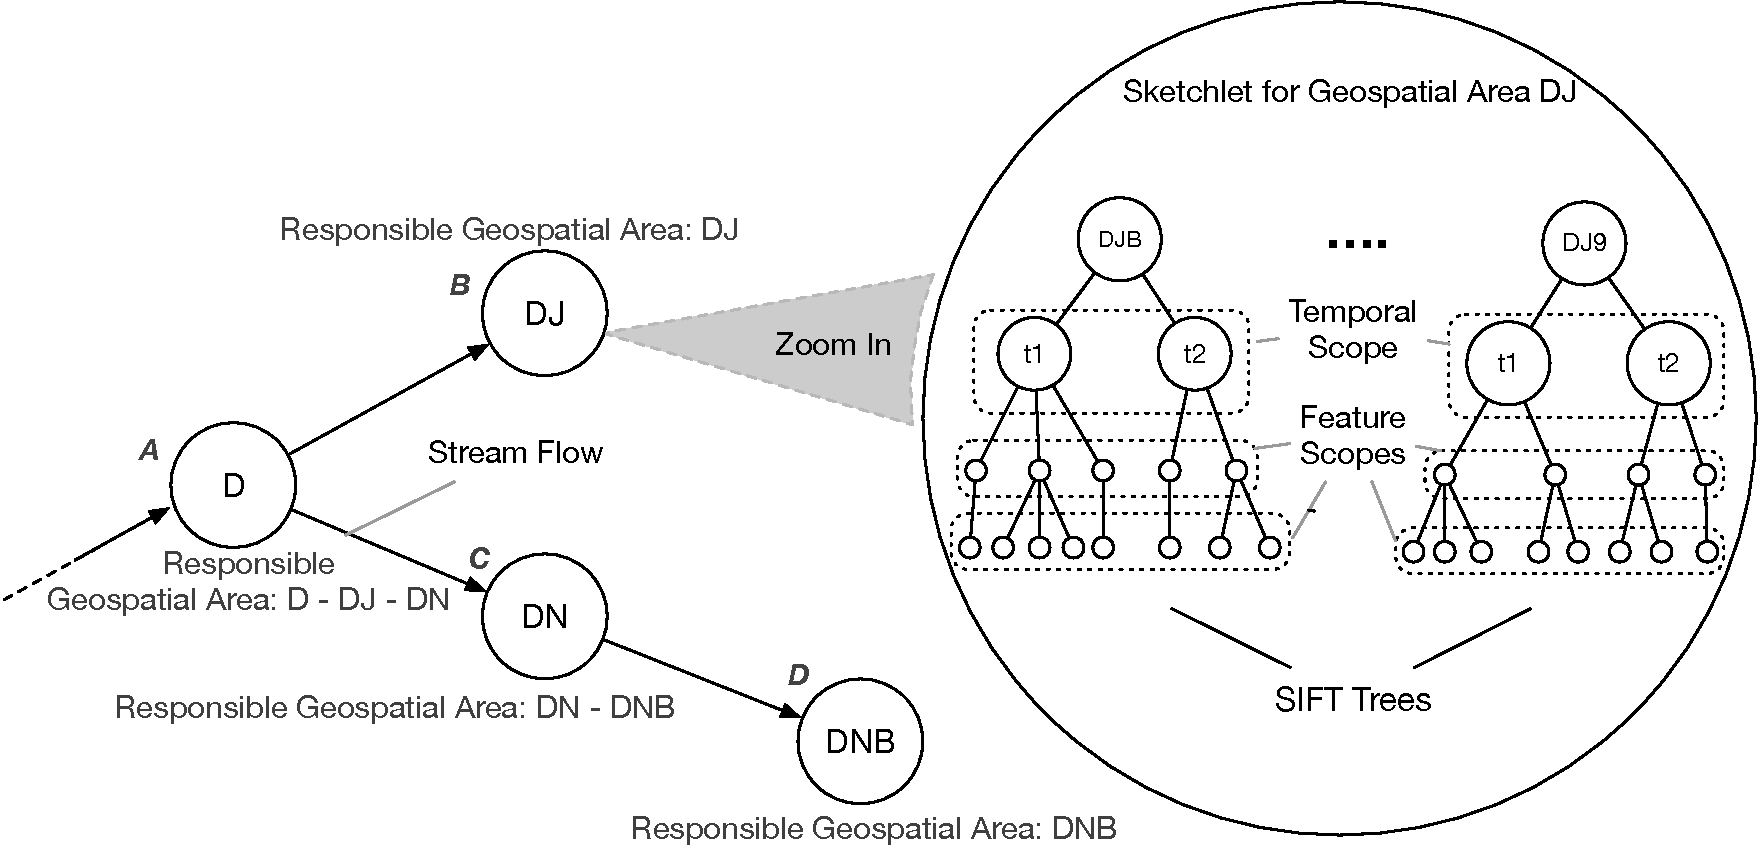
\includegraphics[width=0.5\textwidth]{figures/dist-sketch.pdf}}
    \caption{A demonstration of the distributed sketch for geohash prefix D. The sketchlets for prefixes DJ and DN have scaled out due to high volume of observations. Each sketchlet maintains a SIFT, with each tree responsible for a geospatial subregion. \vspace{-1em}}
    \label{fig:dist-sketch}
\end{figure}

The second level of the SIFT is used to group observations based on their temporal properties. This approach allows us to exploit similarity in readings reported for a particular time range. Note that as the trees are traversed, this organization strategy means that all descendants of a temporal node correspond to measurements reported for a particular region and for a particular temporal scope. The SIFT data structure also supports finer-grained temporal resolutions for the recent past -- e.g., minutes, hours, day, weeks, etc. -- along with targeted compaction operations that fold finer-grained temporal scopes into a coarser grained scopes as time advances. Specifically, our organizational structure allows us to support varying levels of expressiveness for different temporal scopes, with recent observations being represented more expressively.

The grouping concept also extends to individual features. Each feature occupies a level within an individual tree in SIFT. At each level, the range of values that a feature can take is broken up into a set of bins (corresponding to the range of values) that they take. These ranges are determined using kernel density estimation (KDE) to ensure that the binning of features is representative of the observed density in the distribution of values for that feature at the particular spatiotemporal scope. Each node (or bin) maintains the min, max, standard deviation, mean, and the total number of observations it is responsible for.  This is useful during the creation of synthetic datasets that are representative of the observational space for a particular spatiotemporal scope.

The methodology behind SIFT accomplishes two key objectives: first, it captures the distribution of feature values across a spatiotemporal scope. Second, it supports targeted reductions in the observational data volumes while being representative of the observed feature values. This is in contrast to a random sampling scheme, which may be unable to recreate distributions with high fidelity for arbitrary spatiotemporal scopes.

The organization of the sketchlet is such that it is amenable to scale-out and scale-in operations of the distributed sketch. A key feature provided by the SIFT data structure is support for scaling operations. For example, if a subregion represented by a tree within the forest maintained at each sketchlet has a higher density (and variability) of the reported observational values, that tree would have a correspondingly higher memory footprint within the data structure. This allows us to target scaling maneuvers to particular subregions managed at a sketchlet to alleviate memory pressure.  During scale-in operations, descendants can be folded into the parent; the descendant's SIFT is simply added as a tree to the SIFT maintained at the parent.
%
\vspace{0.7em}\\
%
\textbf{Systems View of the Sketch:} The \textsc{Synopsis} sketch, comprising sketchlets dispersed over multiple machines, is a compact and memory-resident surrogate for the entire observational space. The sketch may be used for any purpose that regular, on-disk data is used for including but not limited to query evaluations, assessing statistical properties of the data, and launching computations using well-known analytical engines. The sketch is adaptive and evolves over time, with the number of sketchlets varying as scaling maneuvers occur to cope with data volumes and memory management. The structure of the SIFT also varies over time as temporal scopes are aggregated, features binned, and scaling occurs.

\subsection{Sketchlet}
\label{sec:sketch}
Sketchlets maintain compact, multidimensional, tree-based representations of incoming data streams in the SIFT data structure. Each in-memory SIFT can be queried to retrieve statistical properties about the underlying data or discover how features interact. Due to the voluminous nature of these data streams, storing each record in main memory is not practical. Therefore, the queries supported by our framework are facilitated by compact, online metadata collection and quantization methods. These techniques ensure high accuracy while also conforming to the memory requirements of the system. To further improve accuracy, we bias our algorithms toward the most recent data points while reducing the resolution of the oldest.

\subsubsection{SIFT Structure}
\label{sec:sift}
SIFT instances are maintained as hierarchical trees with feature values stored in the vertices. Each level of the hierarchy, called a \emph{plane}, represents a particular data type, and traversing through vertices in this feature hierarchy incrementally reduces the search space of a query. Upon insertion of a multidimensional observation, each feature is arranged to form a \emph{path} through the tree and added based on the current feature hierarchy. Paths taken through the tree during a lookup are influenced by the specificity of the query, with additional feature expressions constraining the \emph{query scope}; an empty query would result in a scope that spans the entire tree. Figure~\ref{fig:sketch} demonstrates the structure of a SIFT tree and highlights a query and its scope. SIFT trees are internally arranged as modified red-black trees, resulting in lookup and insertion complexities of $O(log\ n)$.

\begin{figure}[b!]
    \centerline{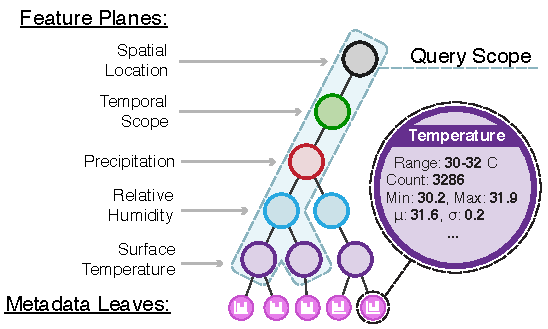
\includegraphics[width=3.2in]{figures/sketch.pdf}}
    \caption{A simplified SIFT tree with five planes and a sample query scope. In production settings, these trees contain hundreds of thousands of vertices and edges.}
    \label{fig:sketch}
\end{figure}

Metadata records for paths through the feature hierarchy are stored at leaf nodes. Each record contains statistics that are updated in an online fashion using Welford's~method~\cite{welford1962note}. Welford's method maintains the number of observations, $n$, the running mean, $\bar{x}$, and the sum of squares of differences from the current mean, $S_n$, as in the following recurrence relation:
\begin{align*}
    \bar{x}_0 &= 0, S_0 = 0 \\
    \bar{x}_n &= \bar{x}_{n - 1} + \frac{x_n - \bar{x}_{n - 1}}{n} \\
    S_n       &= S_{n - 1} + (x_n - \bar{x}_{n - 1})(x_n - \bar{x}_n)
\end{align*}
Besides the observation count and running mean, this enables calculation of the variance and standard deviation of the observed values: $\sigma^2 = \frac{S_n}{n} \hspace{0.5em};\hspace{0.5em} \sigma = \sqrt{{S_n}/{n}}$. Our implementation of Welford's method also maintains the sum of cross products between features to track cross-feature relationships, such as the correlation between temperature values and humidity. Leaf nodes may also be \emph{merged} to combine their respective summary statistics into a single aggregate summary, which allows queries to be evaluated across multiple sketchlets and then fused into a single, coherent result.

\subsubsection{Structural Compaction}
The number of unique feature types stored in the SIFT directly influences the size of the hierarchy, which impacts memory consumption. However, memory use can be managed by manipulating the hierarchical configuration of the trees to increase vertex reuse.  In general, features that exhibit high \emph{fan-out} (many outgoing edges leading to the next level of the hierarchy) should be placed near the bottom of the tree to reduce its overall size. Listing~\ref{lst:fan-out} demonstrates how the fan-out score is calculated.

\begin{lstlisting}[language=Python,style=custompy,emph={fan_out_score,compact_hierarchy},caption={Calculation of the fan-out score (average number of outgoing edges) for dynamic reconfiguration.},label={lst:fan-out}]
def fan_out_score(feature):
    sc = Synopsis.context()
    # Select all vertices for this feature
    vertices = sc.query('SELECT ' + str(feature))
    edges_out = 0
    for vertex in vertices:
        edges_out += vertex.num_neighbors()
    fan_out = edges_out / len(vertices)
    return fan_out
\end{lstlisting}

To illustrate this concept, consider both a boolean feature and spatial location being used as the root of the tree. With the boolean feature, two possible partitions of the tree are created. However, using the spatial location leads to the creation of hundreds or thousands of subtrees, depending on the geohash resolution being used at the sketchlet. This leads to low vertex reuse. Consequently, we \emph{compact} the logical representation of the SIFT by aggregating vertices from the entire forest and reorienting the planes to conserve memory. Listing~\ref{lst:reconfigure} presents the feature plane compaction algorithm.

\begin{lstlisting}[language=Python,style=custompy,emph={fan_out_score,compact_hierarchy},caption={Feature plane compaction algorithm; the hierarchy is reconfigured based on sorted fan-out scores.},label={lst:reconfigure}]
def compact_hierarchy():
    sc = Synopsis.context()
    scores = []
    for feature in sc.features:
        fan_out = fan_out_score(feature)
        scores.append((fan_out, feature))
    new_hierarchy = sort_ascending(scores)
    return new_hierarchy
\end{lstlisting}

One notable result of this process is that vertices near the bottom of the hierarchy may be responsible for storing spatial locations of the data points rather than the root of the tree as depicted in our conceptual model of the SIFT.  After reconfiguration, the fan-out scores are leveraged to estimate the lower and upper bounds for memory usage (the reversed configuration will yield the highest memory consumption).

\subsubsection{Density-Driven Quantization}
Maintaining data points, statistics, and cross-feature relationships in memory at full resolution is infeasible when faced with voluminous datasets, even when load is balanced over several computing resources. To reduce the memory consumption of SIFT instances we perform \emph{quantization} --- targeted reduction of resolution --- which allows vertices in the tree to be merged, thus enabling single vertices to represent a collection of values. We determine which vertices should be merged by splitting each range of feature values into a configurable number of \emph{bins}. After quantization, each vertex represents a range of observations.

To determine the size and quantity of these bins, trees within the SIFT maintain additional metadata provided by the multivariate online kernel density estimation (oKDE) algorithm developed by Kristan et al. \cite{kristan2011multivariate}. While it is possible to recompute kernel density estimates periodically for each feature type using in-memory samples \cite{malensek2013autonomously}, the online approach afforded by oKDE requires less overall CPU usage and memory, which is crucial in streaming environments.  oKDE assimilates data incrementally at runtime to create a dynamic probability density function (PDF) for each feature type. The smoothing parameter used to create the PDF, called the \emph{bandwidth}, is selected autonomously using Silverman's rule \cite{silverman1986density}. Silverman's rule assumes that data tends to follow a normal distribution, which is generally true for naturally-occurring observations. However, we also allow the smoothing parameter be selectively reconfigured for different problem types.

During the quantization process, these PDFs are used to ensure that each bin is assigned an approximately equal proportion of the feature density to create small, highly-accurate bins, while the overall number of bins is influenced by memory availability. Given a PDF and bin count for a feature, our quantization algorithm iterates through the bins and assigns them each an equal portion of the probability density. This process has a time complexity of $O(n)$ where $n$ is the number of bins, but it is worth noting that $n$ is generally small (around 30 on average) and the algorithm is not run frequently.

Figure~\ref{fig:quantization} illustrates the quantization process for the \emph{surface temperature} feature in our atmospheric test dataset \cite{noaa_nam}: the highest densities of values are stored in the smallest bins (indicated by vertical lines under the curve), improving overall accuracy. To evaluate accuracy, we compare the mean values of each bin with the actual, full-resolution data points. Consequently, the \emph{standard error} ($\sigma_{\bar{x}}$) can be calculated from our running summary statistics to judge the accuracy level of the bins based on how well they represent the mean: $ \sigma_{\bar{x}} = \sqrt{{S_n}/{n^2}} $.
%
\begin{figure}[b!]
    \centerline{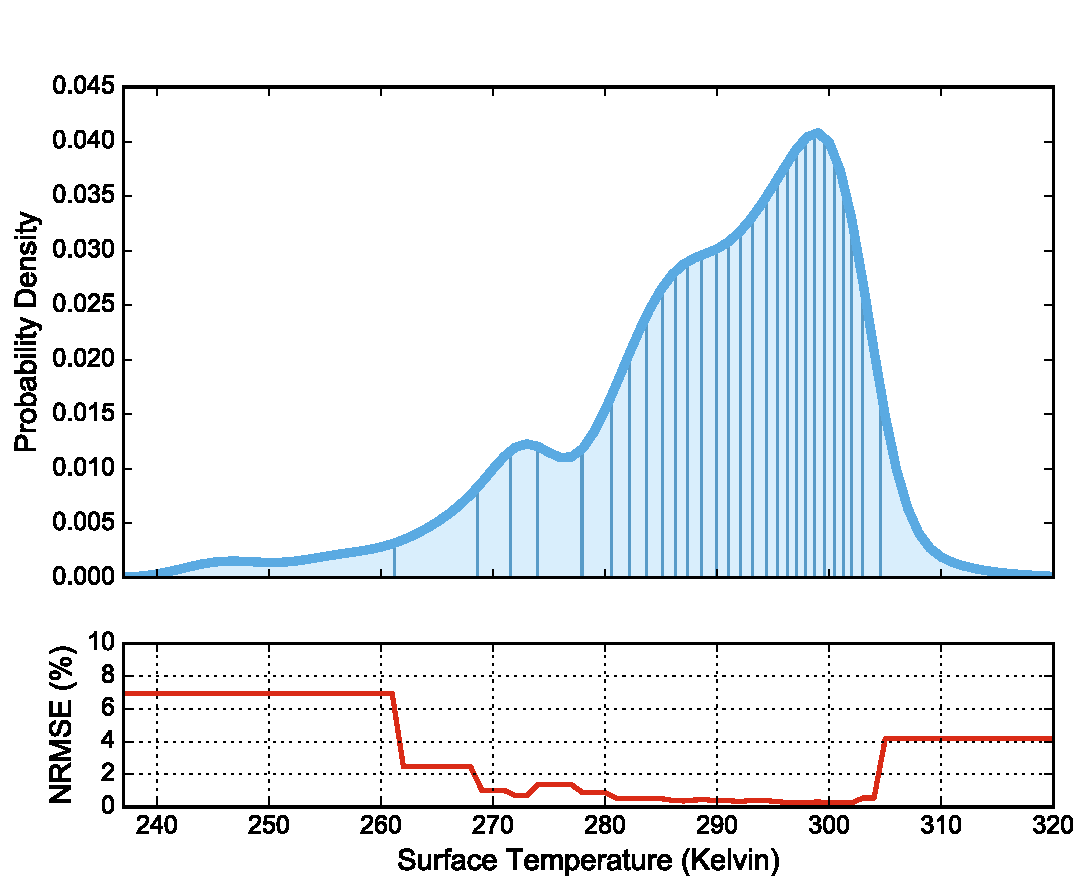
\includegraphics[width=3.5in]{figures/quantization.pdf}}
    \caption{Quantized surface temperatures, with 29 vertex bins. Each bin is indicated by a vertical line under the curve.}
    \label{fig:quantization}
\end{figure}
%
This information is provided alongside any query results returned by the system. During initialization, we calculate the normalized error for each data point empirically (shown in the lower portion of Figure~\ref{fig:quantization}). For values that are observed less frequently, the error rate is higher; temperatures from 240 -- 260 Kelvin (-33.15 to -13.15 \degree C) reach a normalized root-mean-square error (NRMSE) of about 7\%. However, approximately 80\% of the values in the tree will be assigned to vertices with an error of about 0.5\%. In practice, this means that commonly-observed values will be within 0.25 Kelvin of their actual value.

Table~\ref{tbl:tree-stats} compares full-resolution and quantized trees generated from a month of data with 20 unique features, which include atmospheric information such as temperature, humidity, precipitation, and cloud cover. In this configuration, our quantization algorithm reduced memory consumption by about 62.4\%, which allows much more historical data and larger geographical areas to be maintained in each SIFT.
%
\begin{table}[h!]
    \renewcommand{\arraystretch}{1.2}
    \caption{Tree statistics before and after our dynamic quantization algorithm over one month of ingested data.\vspace{-1em}}
    \label{tbl:tree-stats}
    \begin{center}
        \begin{tabular}{|l|c|c|c|}
            \hline
            \textbf{Metric} & \textbf{Original} & \textbf{Quantized} & \textbf{Change} \\
            \hline
            Vertices & 3,104,874 & 1,238,424 & -60.1\% \\
            \hline
            Edges    & 3,367,665 & 1,441,639 & -57.2\% \\
            \hline
            Leaves   & 262,792   & 203,216   & -22.7\% \\
            \hline
            Memory   & 1,710.6 MB & 643.1 MB  & -62.4\% \\
            \hline
        \end{tabular}
    \end{center}
\end{table}

\vspace{-2em}

\subsubsection{Temporal Dimensionality Reduction}
While our quantization approach enables \textsc{Synopsis} to retain large volumes of data in main memory, we also offer a temporal \emph{accuracy gradient} to ensure the most relevant data points are prioritized for high accuracy. This is achieved by iteratively removing tree paths from the SIFT hierarchy in the oldest subtrees, eventually phasing out old records. As data ages, this process results in the creation of temporal accuracy bands.

Selective temporal dimensionality reduction proceeds in a bottom-up fashion, starting from the bottom of the hierarchy. Given a set of relevant vertices, neighboring bins are merged uniformly across the feature space. As the bins are merged, their respective metadata is also merged, reducing memory consumption. Given two metadata instances, merging results in half the memory footprint. However, it is worth noting that this process is irreversible; once metadata has been merged, it cannot be split at a later point in time. As time passes, entire portions of the feature space are compacted until a single metadata record is left for a particular temporal range. This allows users to still query the summary statistics and models for historical data, but at a lower level of accuracy.

\subsubsection{Facilitating Scalability}
The SIFT is designed to facilitate distribution across several computing resources. Specifically, splitting and merging functionality is exposed via the same query interface used for resolving user requests. Queries proceed in a depth-first fashion, locating a \emph{subtree root} within the hierarchy. Once the root is established, either: (1) its descendants are serialized for transmission to another sketchlet, or (2) an incoming subtree is merged in place. During merges, existing paths are reused with only leaf nodes requiring updates.

\subsection{Coping with High Loads: Scaling out}
\label{subsec:scaling-out}
%
\begin{figure}[h!]
    \centering
    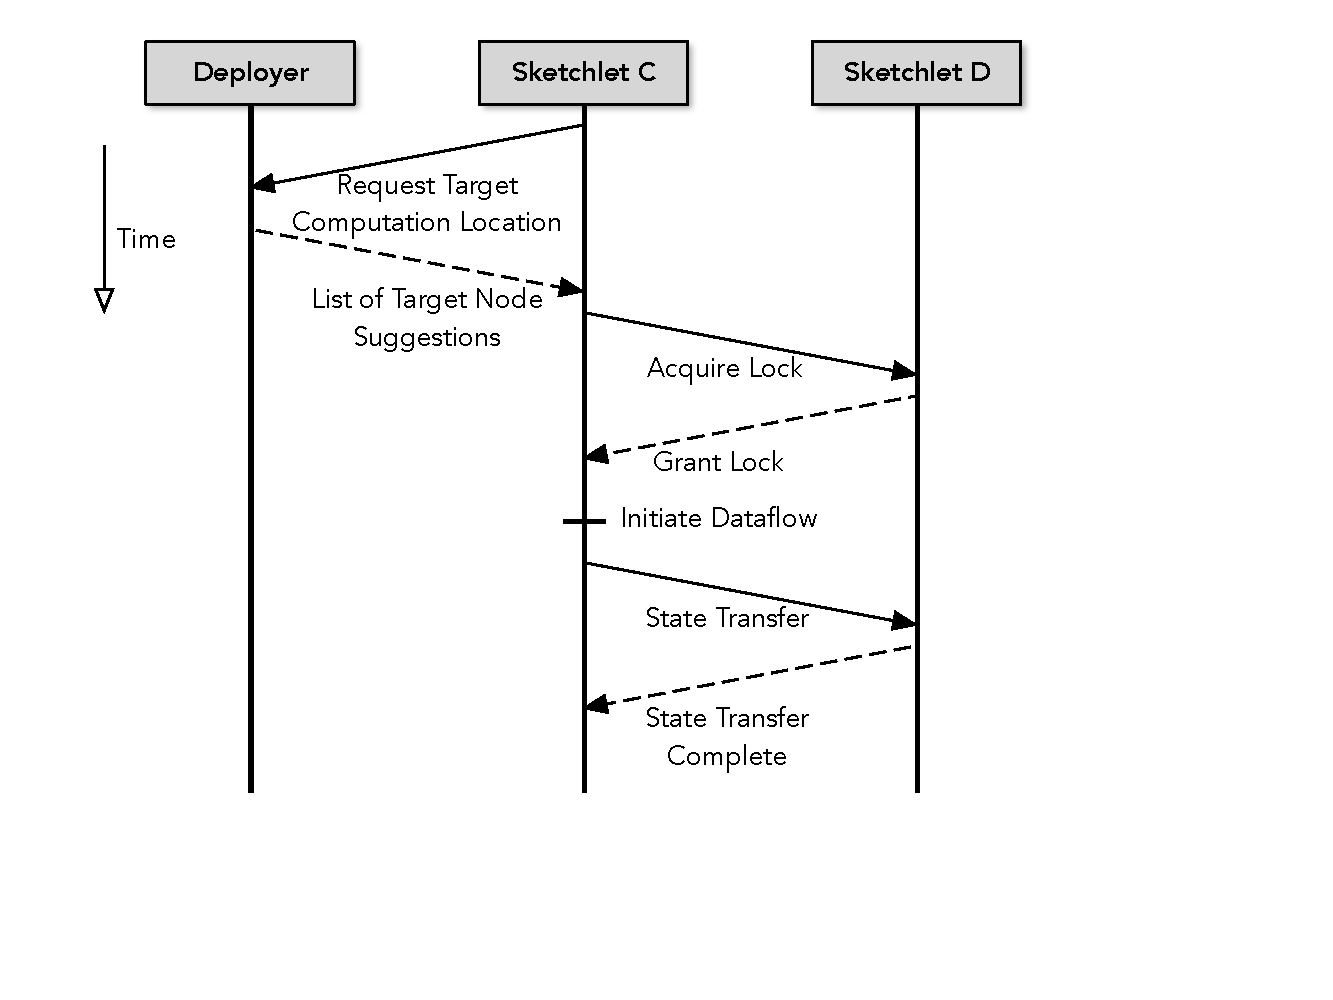
\includegraphics[scale=0.4, valign=t]{figures/scale-out.pdf}
    \caption{Scale-out protocol}
    \label{fig:scale-out-protocol}    
    \vspace{-1em}
\end{figure}
There are two primary approaches to scaling a sketchlet that is experiencing high load: \emph{replication} and \emph{load migration}. In replication-based scaling, new sketchlets are spawned during high data arrival rates that are responsible for identical spatial scopes as their originating sketchlet. Assimilation of the newly-created sketchlet involves partitioning inbound streams directed to the original sketchlet. The upstream node (e.g., stream ingester) is responsible for partitioning, which may be performed in a skewed fashion with the new sketchlet receiving a larger portion of the inbound stream. Alternatively, inbound streams to the original sketchlet may also be partitioned in a round-robin fashion between the original and the newly-created sketchlet.
Using a replication-based scaling with a round-robin style stream partitioning is memory inefficient because of the possibility of multiple SIFT trees with significantly overlapping sets of vertices and edges. Alternatively, \emph{targeted} load migration selects geospatial scopes that are experiencing heavy load; both data arrival and SIFT update rates are considered when deciding which trees to migrate.

In \textsc{Synopsis}, we use targeted load migration for scaling out.
Our implementation closely follows the MAPE loop~\cite{maurer2011revealing} which comprises four phases: monitor (M), analyze (A), planning (P) and execution (E).
A \textbf{monitoring} task within every sketchlet periodically gathers two performance metrics:
\begin{enumerate}[leftmargin=*]
    \item \textbf{Length of the backlog:} This represents the number of unprocessed messages in the queue. If the sketchlet cannot keep up with the incoming data rate, the backlog grows.
    \item \textbf{Memory pressure:} Each sketchlet is allocated a fixed amount of memory. 
    Exceeding these memory limits creates memory pressure causing extended garbage collection cycles and increased paging activity, eventually leading to reduced performance.
    The monitoring task continuously records memory utilization and triggers scaling activities.
\end{enumerate} 

The objective of scaling out is to maintain \emph{stability} at each sketchlet.
We define stability as the ability to keep up with incoming data rates while incurring a manageable memory pressure.  During the \textbf{analyze} phase, we use threshold-based rules \cite{lorido2012auto} to issue scale-out recommendations to sketchlets, which are issued if \textit{either} of the following rules are consistently satisfied for a certain number of monitoring cycles:
\begin{itemize}[leftmargin=*]  
\item Backlog growth, which indicates that a portion of the load needs to be migrated to a different sketchlet.
\item High overall memory utilization above a threshold, which is usually set below the memory limits to allow a capacity buffer for the process to avoid oscillation.
\end{itemize}
Upon receiving a scale out recommendation during monitoring, the sketchlet executes the \textbf{planning} and \textbf{execution} phases.

During the planning phase, the sketchlet chooses portion(s) of the region within its current purview, i.e. a set of SIFT trees, to be handed over to another sketchlet.
For this task, it relies on performance metrics it maintains for each subregion and a numeric value provided by the scale-out recommendation that measures how much load should be migrated.
These metrics includes the data rate and the memory consumption for each subregion.
If the backlog growth based threshold rule has triggered the scale out operation, the subregion metrics are sorted based on their update rates in the descending order. Otherwise they are sorted based on their memory consumption.
Then a simple bin-packing algorithm is used to choose a minimum set of subregions for migration such that the excess load is removed from the current sketchlet.

Only a single scaling operation takes place at a given time per sketchlet, which is enforced by a mutex lock.
Further, every scaling operation is followed by a \textit{stabilization period} where no scaling operation takes place and system does not enter the monitoring phase for the next MAPE cycle.
The objective of these constraints is to avoid oscillations in scaling activities; for instance, repetitively scaling out in the presence of memory pressure could result in overprovisioning, which would then lead to recurring scale-in operations.
%

Figure~\ref{fig:scale-out-protocol} depicts the phases of the scale-out protocol with respect to our example in Figure~\ref{fig:dist-sketch} when sketchlet C is scaling out to sketchlet D.
Once the sketchlet decides on subregions to scale, it initiates the scale-out protocol by contacting the \emph{deployer} process, which is responsible for launching tasks.
In this message, it includes a list of preferred target sketchlets for the load migration as well as memory requirements and expected message rate for the load.
The preferred sketchlet set includes the sketchlets that already hold other subregions.
It minimizes the number of sketchlets responsible for each geographical region to reduce communication during query evaluations.
% system stability
\begin{figure*}[h!]
    \begin{subfigure}{0.48\textwidth}
            \centering
            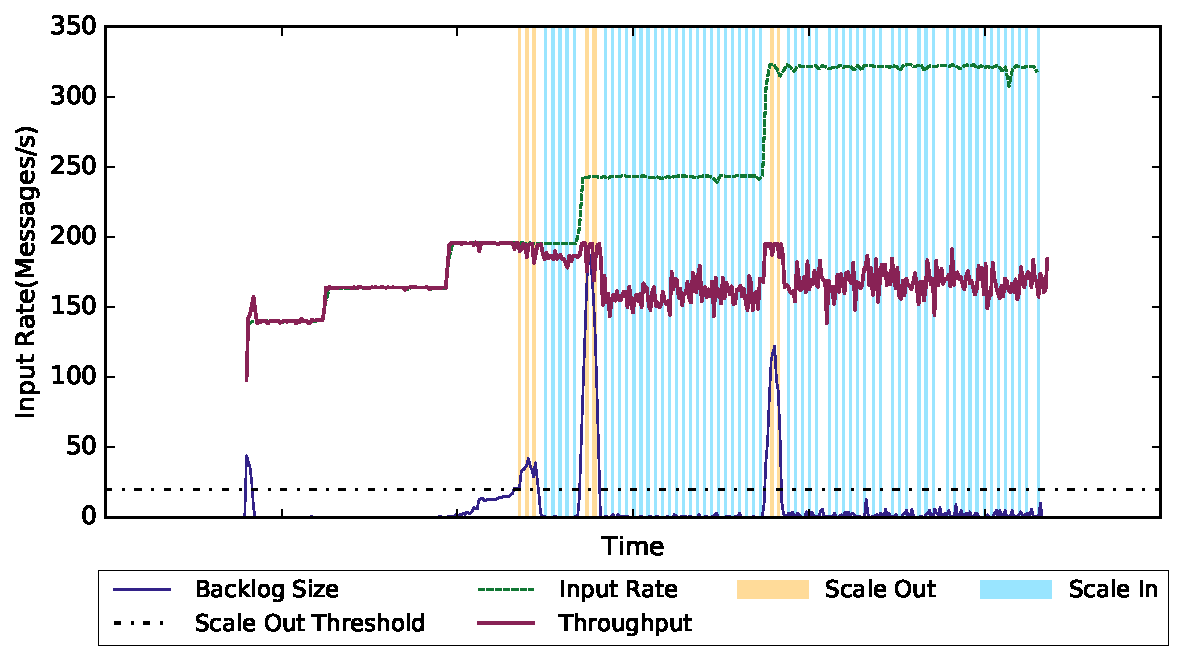
\includegraphics[scale=0.42]{figures/stability_partial.pdf}
            \caption{Triggered by backlog growth based threshold rules}
            \label{fig:stability-backlog}
    \end{subfigure}
    \begin{subfigure}{0.48\textwidth}
            \centering
            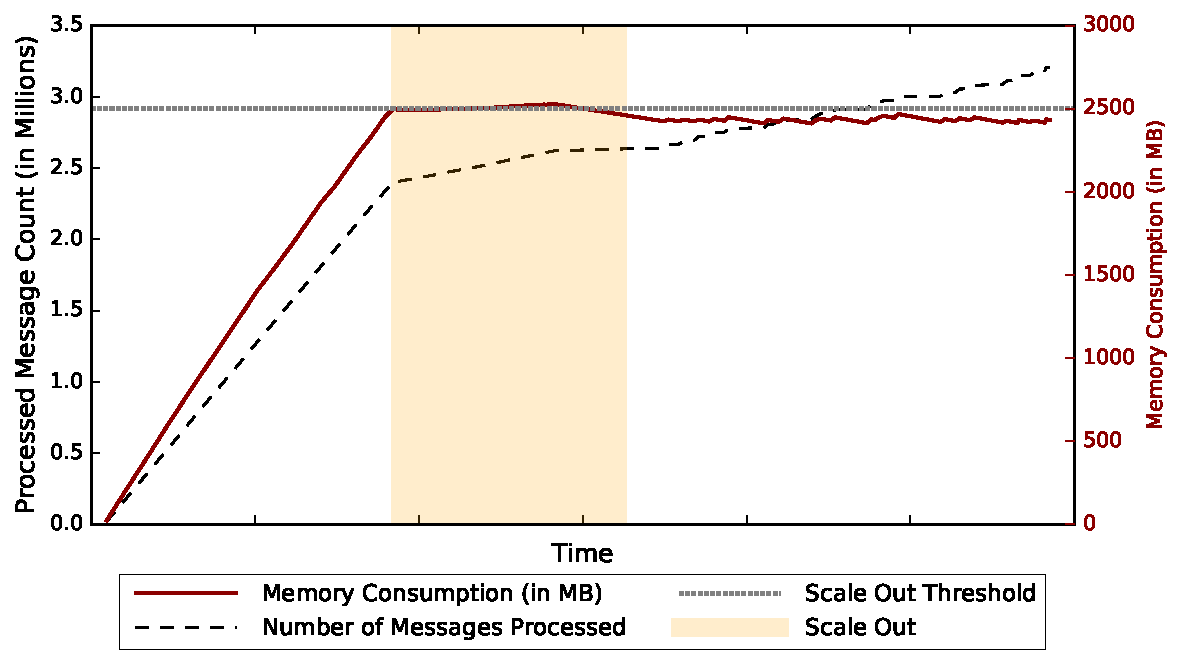
\includegraphics[scale=0.42]{figures//mem_stability.pdf} 
            \caption{Triggered by memory usage based threshold rules}
            \label{fig:stability-mem}
    \end{subfigure}
    \vspace{-.5em}
    \caption{Scaling out based on backlog growth and memory usage enables maintaining stability at an individual sketchlet}
    \label{fig:system-stability}
    \vspace{-1.5em}
\end{figure*}
%
The \textsc{Synopsis} deployer component has an approximate view of the entire system constructed through gossip messages. This includes the memory pressure and cumulative backlog information for each sketchlet.
Based on this view and the information present in the request, the deployer replies back with a set of candidate target sketchlets.
Only if a suitable candidate cannot be found from the set of current sketchlets will a new sketchlet be spawned.
Upon receiving a response from the deployer, the sketchlet (parent) contacts the target sketchlet (child) and tries to acquire the mutex.
A lock will be granted only if the target can accommodate the load and no other scaling operations are taking place.
If the lock acquisition fails, another candidate from the list is attempted; otherwise, the parent sketchlet will create a pass-through channel and direct traffic corresponding to migrated regions towards the child sketchlet.
Once this process is complete, the parent sketchlet will initiate a state transfer asynchronously using a background channel to ensure the stream data flow is not affected, and update the child sketchlet's memory utilization metrics to account for the pending state transfer.

As the data flow tree grows with scale-out operations, having parent sketchlets pass traffic through to their children becomes inefficient because of higher bandwidth consumption as well as increased latency due to the additional network hops the packets have to traverse through.
To circumvent this, we allow \emph{short circuiting}, which redirects traffic from stream ingesters straight the downstream sketchlets.
For instance, stream ingesters will send data directly to sketchlet D using the short circuited route bypassing sketchlets A and C in Figure~\ref{fig:dist-sketch}. 
We use our gossiping subsystem to update parent sketchlets about the child's performance metrics required for scaling in (\S\ref{subsec:scaling-in}).

We evaluated how each of these rules triggers dynamic scaling activities to maintain the system stability.
For this experiment, we have enabled only a single threshold-based rule at a time to demonstrate its effectiveness.
To evaluate the backlog based threshold rule, we captured how backlog length and throughput at an individual sketchlet varies with the input rate.
The sketchlet immediately received data from stream ingesters, hence the input rate observed at the sketchlet closely resembled the varying data ingestion rate.
As shown in Figure~\ref{fig:stability-backlog}, scaling out helps a sketchlet to keep pace with the variations in the workload, which in turn causes the backlog to stay within a safe range.
This benchmark also shows infrequent, rapid scale-out and continuous, gradual scale-in as explained in \S\ref{subsec:scaling-out}.

Figure~\ref{fig:stability-mem} demonstrates how memory consumption threshold rules trigger scaling maneuvers to maintain the stability of an individual sketchlet.
We have used 0.45 of the total memory available to a JVM process as the upper threshold for triggering scale-out operations.
In certain occasions, it is required to perform multiple consecutive scaling out operations (interleaved with the cooling down periods) to bring memory usage to the desired level due to the increased utilization caused by background data ingestion. \vspace{-1em}

%
%
\begin{figure}[b!]
    \centering
    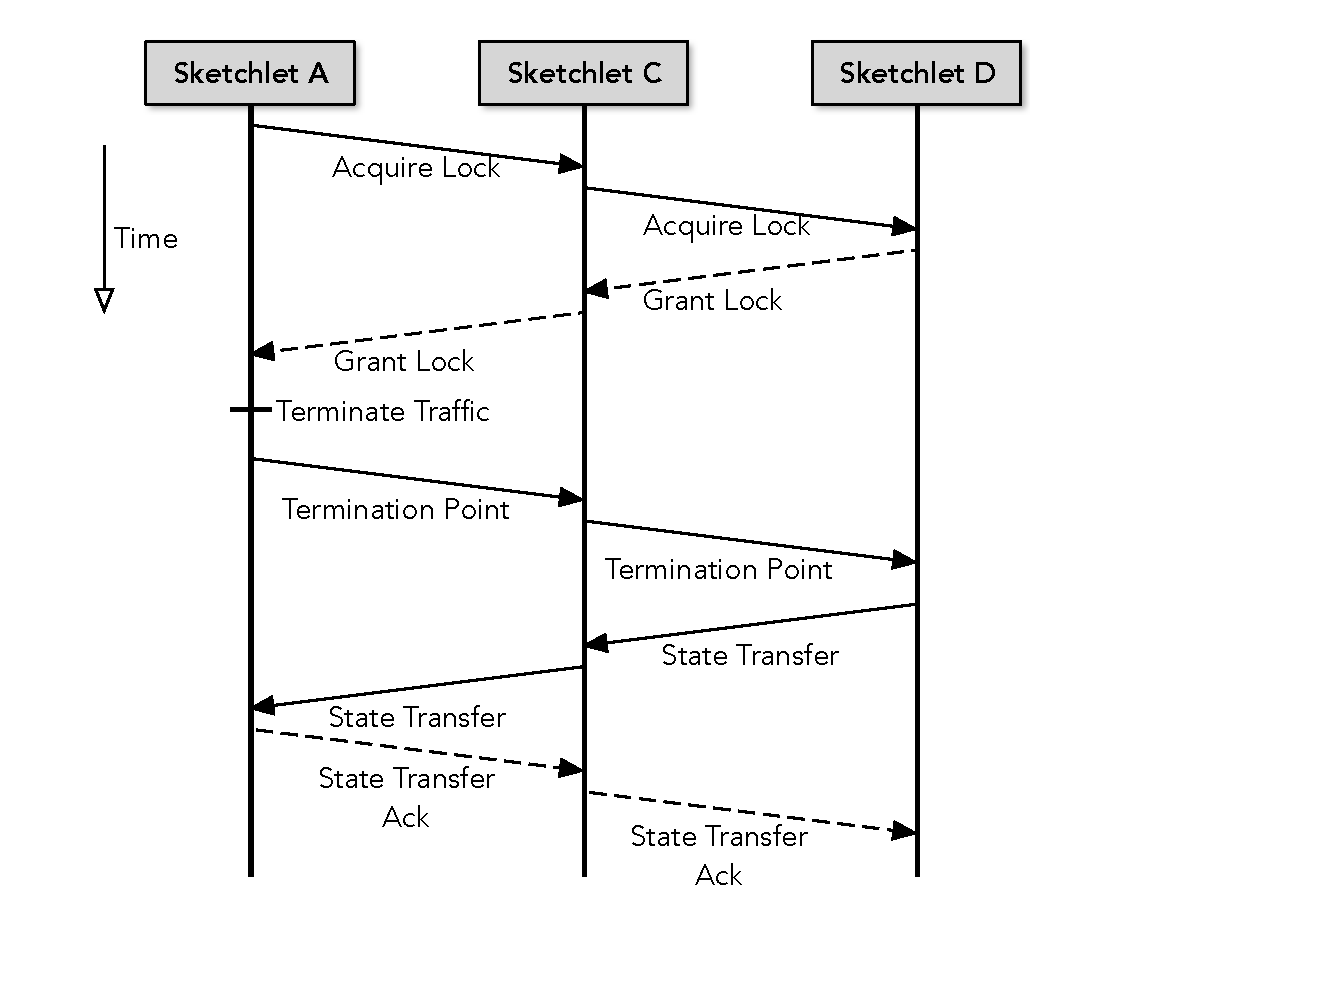
\includegraphics[scale=0.4, valign=t]{figures/scale-in.pdf} 
    \caption{Scale-in protocol}
    \label{fig:scale-in-protocol}
\end{figure}
\subsection{Scaling In: Conserving Resources}
\label{subsec:scaling-in}
During scaling in, sketchlets merge scaled-out subregions back into their SIFT.
This ensures better resource utilization and reduces the number of sketchlets contacted during query evaluations.
Scaling in is also guarded by the same mutex used for scaling out and is also followed by a stabilization period.

Monitoring and analysis during scale-in operations proceeds similarly to scaling out, except for the obvious change to the threshold-based rules: now \textit{both} memory pressure and backlog length metrics should consistently record values below a predefined lower threshold.
When scaling in, we use a less aggressive scheme than scaling out; a single subregion is acquired during a single scale-in operation.
Scaling in is more complex because it involves more than one sketchlet in most cases; 
at this point, it is possible that further descendant scale-out operations have taken place.
For instance, if sketchlet A in Figure~\ref{fig:dist-sketch} decides to scale in subregion \emph{DN}, then it must communicate with sketchlets C and D.

The scale-in protocol starts with a lock acquisition protocol similar to the scaling out protocol, but involves locking the entire subtree.
The steps are depicted in Figure~\ref{fig:scale-in-protocol} with respect to our example in Figure~\ref{fig:dist-sketch} where sketchlet C is scaled in.
As per our example, sketchlet A will acquire locks for both sketchlets C and D.
Locks are acquired in a top-to-bottom fashion where parent locks itself and then attempts to lock the child.
If lock acquisition fails for any part of the subtree, the scale-in operation is aborted and the monitoring process starts the next iteration of the MAPE loop immediately.
If the lock acquisition is successful, then data flow to the child sketchlet corresponding to this subregion is immediately terminated.

The state acquisition phase begins next.
To ensure that \textsc{Synopsis} does not lose any messages, the initiating sketchlet sends a \emph{termination point} control message to the child sketchlet.
The termination point is the sequence number of the last message sent to the child sketchlet either by the parent itself or by the short circuit channel.
Once the child sketchlet has processed every message up to the termination point, it sends out termination point messages to all relevant child sketchlets. In our example, sketchlet C sends a termination point control message to D upon processing the stream packet corresponding to the termination point sent by sketchlet A.
After the entire subtree has seen all messages up to the termination point, they acknowledge the initiator sketchlet and start transferring their states asynchronously.
Once the parent sketchlet receives acknowledgments from the entire subtree, it propagates the \emph{protocol end} messages to release locks.
Locks are released from the bottom to top in the subtree, with the parent sketchlet releasing its lock after each child has released its lock.
%
\subsection{Query Evaluations}
\label{subsec:query-eval}
\textsc{Synopsis} incorporates support for user-defined queries that are evaluated over the distributed sketch.  Queries can be specified by the user in a SQL-like format or with JSON-based key-value descriptions similar to GraphQL~\cite{graphql}. Exact-match, range-based, and summarization queries are all supported over spatiotemporal bounds and individual feature values. The following example depicts how SQL-like queries can be formulated for evaluation over the sketch.

\begin{lstlisting}[language=SQL,style=custompy]
    SELECT MEAN(precipitation), MAX(wind_speed)
    WHERE temperature > 20 AND temperature < 30
    AND humidity > .8 AND CORRELATION(
        cloud_cover, precipitation) < -0.25
\end{lstlisting}

Depending on scaling operations and the spatial scope of the queries, evaluations are carried out on one or more sketchlets. Information on the placement of sketchlets in the system and their corresponding feature scopes is maintained at each sketchlet in a geohash prefix tree, with changes propagated through the network in an eventually-consistent manner as data is ingested and scaling maneuvers occur.

The entry point for these queries, called the \emph{conduit}, may be any of the sketchlets comprising the distributed sketch. During query evaluations, the first step is to identify the set of sketchlets relevant to the query. The conduit consults its prefix tree to locate sketchlets based on spatial, chronological, and feature constraints specified by the user. For spatial constraints that overlap multiple geohashes, a set of \emph{minimum bounding geohashes} (MBG) is constructed based on query geometry. Points falling outside the MBG are trimmed at the individual sketchlet level, in a fashion similar to traversing an R-Tree \cite{guttman1984r}.  After this process is complete, the conduit forwards the queries on to the sketchlets for evaluation and supplies the client with a list of responding sketchlets.  As queries execute, results are streamed back and merged by the client API. This strategy ensures that I/O and processing activities are interleaved.

In some situations, a trade-off arises between false positives and false negatives when queries overlap but do not completely cover quantization bins. Users are made aware of this through the error bounds provided by \textsc{Synopsis}, but in cases where false positives are undesirable, partially-matching bins can be pruned from the results. This also affects spatial queries, albeit much less often; while high-resolution geohashes are stored in the SIFT, the encoding scheme is inherently lossy and may produce false positives depending on the configured resolution.

Our distributed prefix tree enables query evaluations during both scaling in and out. For instance, when a conduit attempts to forward a query to a child sketchlet that is undergoing a scale-in operation, the request will be redirected to the its parent sketchlet. This process can continue recursively up through the network, ensuring queries will reach their destination.

\subsubsection{Query Types Supported by \textsc{Synopsis}}
\begin{description}[leftmargin=*]
    \item[Relational Queries] describe the feature space in the context of the hierarchical trees within our SIFT data structure and may target ranges of values; e.g., ``What is the relationship between temperature and humidity during July in Alaska, when precipitation was greater than 1 cm?'' These queries return a subset of the overall sketch.
    % Subsketches may be manipulated and inspected on the client side, and then reused in subsequent queries to request more detail or broaden the query scope. Relational queries can optionally return statistical metadata stored in the leaf nodes of the tree; this is also supported by our statistical query functionality.

    \item[Statistical Queries] allow users to explore statistical properties of the observational space. For example, users can retrieve and contrast correlations between any two features at different geographic locations at the same time. Alternatively, queries may contrast correlations between different features at different time ranges at the same geographic location. These queries also support retrieval of the mean, standard deviation, and feature outliers based on Chebyshev's inequality \cite{knuth1968art}.

    \item[Density Queries] support analysis of the distribution of values associated with a feature over a particular spatiotemporal scope. These include kernel density estimations, estimating the probability of observing a particular, and determining the deciles and quartiles for the observed feature.% Kernel density estimations can request the function itself, an integral over a range of values, or the probability of a single value.

    \item[Set Queries] target identification of whether a particular combination of feature values was observed, estimating the cardinality of the dataset, and identifying the frequencies of the observations. Each type of set query requires a particular data structure, with instances created across configurable time bounds (for instance, every day). Set membership is determined using space-efficient bloom~filters~\cite{bloom1970space}, while cardinality queries are supported by the HyperLogLog~\cite{flajolet2007hyperloglog} algorithm.

%To determine set membership, we use Bloom filters may produce false positives, but never false negatives. Besides returning a \texttt{true} or \texttt{false} result to the user, membership queries also include the probability of the answer being a false positive.  Set HyperLogLog is able to estimate cardinality with high accuracy and low memory consumption. Finally, observation frequencies are provided by the count-min data structure \cite{cormode2005improved}. Count-min is structurally similar to a bloom filter, but can be used to estimate the frequency of values within a particular error band. Frequency queries are accompanied by their associated confidence intervals and relative error.

\item[Inferential Queries] enable spatiotemporal forecasts to be produced for a particular feature (or set of features). Discrete inferential queries leverage existing information in the distributed sketch to make predictions; aggregate metadata stored in the leaves of the tree can produce two-dimensional regression models that forecast new outcomes across each feature type when an independent variable of interest changes.

%In their continuous form, inferential queries are backed by machine learning models that are \emph{installed} for a particular time window and can be trained using either the sketch or new, full-resolution values as they arrive. Continuous inferential queries can stream predictions back to the client on a regular interval, or a subsequent query can reference a particular model and parameterize it to make a single prediction. Our current implementation of \textsc{Synopsis} supports multiple linear regression, but our machine learning interface allows new models to be plugged into the system at run time.

\item[Synthetic Data Queries] allow users generate representative datasets based on the distributions stored in the sketch and then stream them to client applications for analytics. The size of the dataset may also be specified; for instance, 10\% of the volume of the original data points.
\end{description}
%
\begin{table}
    \renewcommand{\arraystretch}{1.2}
    \caption{Local query evaluation times (1000 iterations). \vspace{-1em}}
    \label{tbl:query-times}
    \begin{center}
        \begin{tabular}{|l|c|c|}
            \hline
            \textbf{Query Type}      & \textbf{Mean (ms)} & \textbf{Std. Dev. (ms)} \\
            \hline
            Density                  & 0.007                    & 0.005 \\
            \hline
            Set Cardinality          & 0.154                    & 0.088 \\
            \hline
            Set Frequency            & 0.036                    & 0.019 \\
            \hline
            Set Membership           & 0.015                    & 0.009 \\
            \hline
            Statistical               & 0.002                    & 0.001 \\
            \hline
            \hline
            Tree Only (5 km)        & 46.357                   & 1.287 \\
            \hline
            Tree + Meta (5 km)      & 40.510                   & 6.937 \\
            \hline
            Tree + Meta (25 km)     & 47.619                   & 6.355 \\
            \hline
            Tree + Meta (800 km)    & 53.620                   & 6.818 \\
            \hline
        \end{tabular}
    \end{center}
    \vspace{-2em}
\end{table}
Table~\ref{tbl:query-times} outlines tree traversal times for query evaluations. These queries were separated into two groups: conventional lookups and tree retrievals. Conventional lookups include density queries, set queries, and statistical queries, while tree retrievals request targeted portions of the SIFT.  While conventional lookups do not return a tree structure to the client, they still require a tree traversal to resolve. In general, tree retrievals consume more processing time due to their serialization and I/O costs; however, it is worth noting that varying the geographical scope across sketchlet sizes from 5km to 800km did not result in a proportionate increase in processing time.
\subsection{Coping with Failures in \textsc{Synopsis}}
\textsc{Synopsis} relies on passive replication to recover from sketchlet failures because active replication increases resource consumption significantly and it is infeasible to use upstream backups because the state of a sketchlet depends on the entire set of messages it has processed previously \cite{castro2013integrating}.

Support for fault tolerance is implemented by augmenting the distributed sketch with a set of secondary sketchlets.
A sketchlet is assigned a set of $n$ secondary sketchlets on different machines to ensure \textsc{Synopsis} can withstand up to $n$ concurrent machine failures.
In our implementation, we used two secondary sketchlets ($n=2$) assigned to each sketchlet.
A primary sketchlet periodically sends the changes to its in-memory state as an \emph{edit stream} to its secondary sketchlets.
The secondary sketchlets, which act as the sink to the edit stream, serialize incoming messages to persistent storage.
This incremental checkpointing scheme consumes less bandwidth compared to a periodic checkpointing scheme that replicates the entire state \cite{castro2013integrating}.
By default, \textsc{Synopsis} uses the disk of the machine executing the secondary sketchlet as the persistent storage, but highly-available storage implementations such as HDFS~\cite{borthakur2008hdfs} can be used if necessary.
To reduce resource footprints, secondary sketchlets do not load the serialized state into memory unless they are promoted to being a primary.

System-wide incremental checkpoints are orchestrated by a special control message emitted by the stream ingesters.
\textsc{Synopsis} uses upstream backups at stream ingesters to keep a copy of the messages that entered the system since the last successful checkpoint.
In case of a failure, all messages since the last checkpoint will be replayed.
Sketchlets are implemented as idempotent data structures using message sequence numbers, hence they will process a replayed message only if it was not processed before.
The interval between incremental checkpoints can be configured based on time or the number of emitted messages.
Frequent checkpoints can incur high overhead, whereas longer periods between successive checkpoints consume more resources for upstream backups and require longer replay durations in case of a failure.

Membership management is implemented using Zookeeper~\cite{hunt2010zookeeper}, which is leveraged to detect failed sketchlets.
Upon receiving notification of a primary sketchlet failure, a secondary sketchlet assumes the role of primary through a leader election algorithm.
The secondary will start processing messages immediately and begins populating its state from persistent storage in the background.
Given this mode of operation, there may be a small window of time during which the correctness of queries are impacted.
This is rectified once the stored state is loaded to memory and the replay of the upstream backup is completed.
The SIFT's support for merge operations as well as its ability to correctly process out of order messages is useful during the failure recovery process.

As per our fault tolerance scheme, the \textit{total time to recover from the failure} ($T_{total}$) can be modeled as follows.
\begin{align*}
    T_{total} &= T_{d} + \max{(T_{l}, T_{r})}      
\end{align*}
where $T_{d}$ = \textit{time to detect a failure}, $T_{l}$ = \textit{time to load persisted state} and $T_{r}$ = \textit{replay time for messages at the upstream node}.

The time required to detect failures mainly depends on the session timeout value used by Zookeeper to detect lost members and the delay in propagating the notification to other members. With a $5s$ session timeout in an active cluster, we observed a mean notification propagation delay of $5.5s$ (std. dev. = $0.911s$, $95^{th}$ percentile = $6.000s$). Configuring a lower session timeout will increase the chance of false positives if sketchlets become non responsive for a while due to increased load or system activities such as garbage collection. The time required to load the persisted storage depends on the size of the serialized sketchlet; we benchmarked the time it takes to repopulate the state in all sketchlets after ingesting NOAA data for 2014. The mean state re-population time was recorded as $16.602s$ with std. dev. = $23.215s$ and $95^{th}$ \%ile = $70.877s$. Replay time mainly depends on the checkpointing interval as well as the message ingestion rate. With a checkpointing interval of 10000 messages, we experienced a mean value of $0.662s$ (std. dev. = $0.026s$, $95^{th}$ \%ile = $0.707s$) to replay an upstream buffer.
%
% Evaluation
%
\section{Performance Evaluation}
Here we report system benchmarks profiling several aspects of \textsc{Synopsis}, including the memory consumption and data ingestion performance of the sketch, its ability to handle variable loads, organization of sketchlets, and query performance.
\label{sec:performance}
\subsection{Dataset and Experimental Setup}
We used two datasets for our evaluation.
The first was sourced from the NOAA North American Mesoscale (NAM) Forecast System~\cite{noaa_nam}.  The NAM collects atmospheric data several times per day and includes features of interest such as surface temperature, visibility, relative humidity, snow, and precipitation. The size of this entire source dataset was 25 TB.
The other dataset, collected by the US Environmental Protection Agency, contained daily summary data of four criteria gases ($O_3$, $SO_2$, $CO$ and $NO_2$) used for calculating the air quality in a given area~\cite{epa-criteriagases}. Each observation in both datasets also incorporates a relevant geographical location and time of creation. This information is used during the data ingest process to partition streams across available sketchlets and preserve temporal ordering of events. Data streams were ingested at faster rates to simulate high data arrival rates while ensuring temporal ordering was preserved.

Performance evaluations reported here were carried out on a cluster of 40 HP DL160 servers (Xeon E5620, 12 GB RAM). The test cluster was configured to run Fedora 24, and \textsc{Synopsis} was executed under the OpenJDK Java runtime 1.8.0\_72.
For evaluations involving Apache Spark, we used Apache Spark version 2.0.1 with HDFS 2.6.0 with a 100 node cluster by combining our baseline cluster of 40 machines with 30 HP DL320e servers (Xeon E3-1220 V2, 8 GB RAM) and 30 HP DL60 servers (Xeon E5-2620, 16 GB RAM). 


\subsection{Distributed Sketch Memory Evaluation}
We monitored the growth in memory consumption of the entire distributed sketch over time with continuous data ingestion as shown in Figure~\ref{fig:dist-sketch-mem-usage} for both datasets. As more data was streamed into the system, the growth rate decreased as the sketchlets expanded to include vertices for their particular feature space.  At the end of our monitoring period, the total amount of ingested data was around three orders of magnitude higher ($\sim 1285$ for NOAA data and $\sim 926$ for air quality data) than the in-memory sketch size, resulting in notable space savings.
%
%
\begin{figure*}[t!]
    \centerline{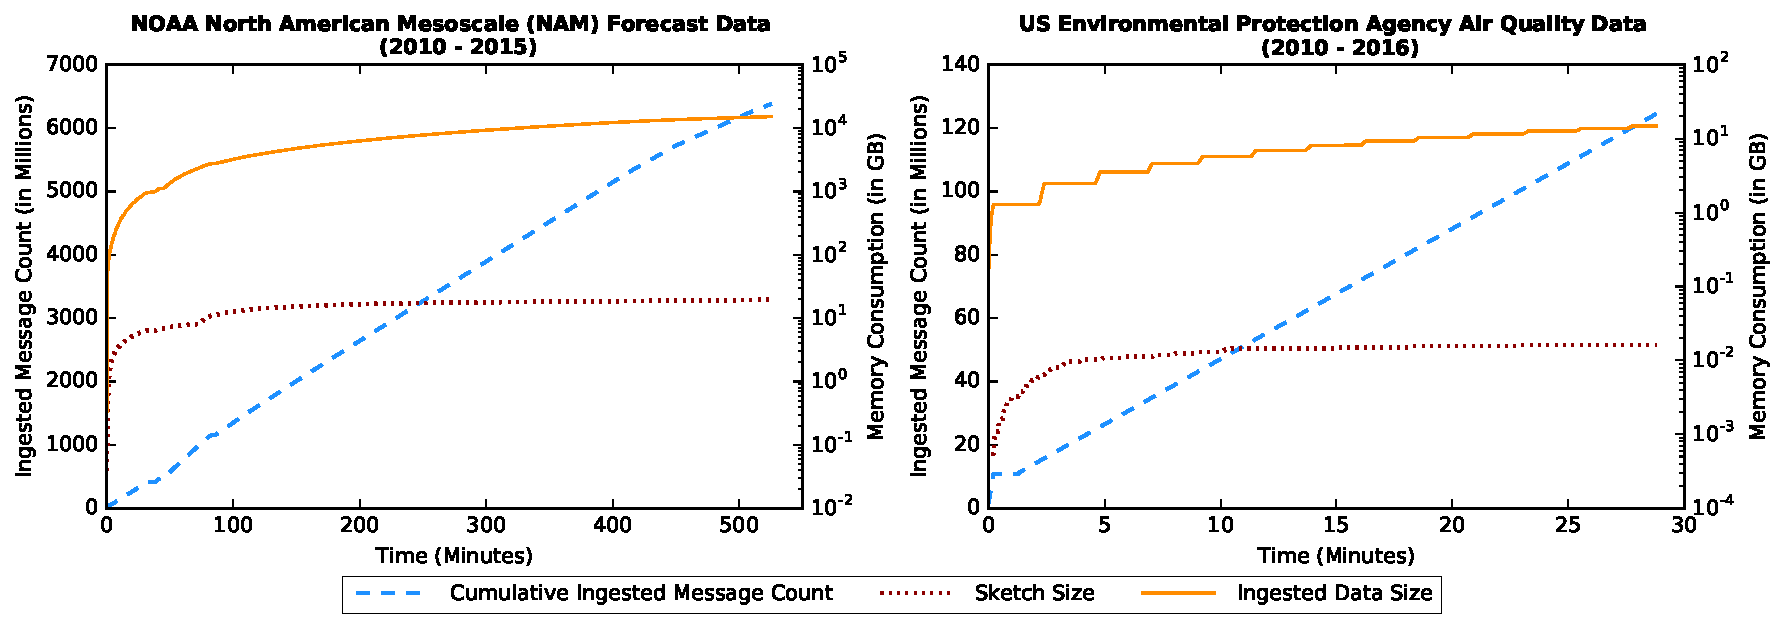
\includegraphics[width=\linewidth]{figures/ing-and-mem-usage-noaa-airquality.pdf}}
    \caption{Memory usage of the distributed sketch over time against the amount of ingested data. The rate of growth decreases over time due to the compact nature of sketchlet data structure.}
    \label{fig:dist-sketch-mem-usage}
\end{figure*}
%
\subsection{Sketch Ingestion Rate}
%
\begin{table*}[bh!]
    \renewcommand{\arraystretch}{1.2}
    \caption{Profiling the update performance of sketchlet and sketch at high data ingest rates}
    \label{tab:throughput}
    \begin{center}
        \begin{tabularx}{0.9\textwidth}{|X|c|c|c|c|c|c|c|}
            \hline
            \multirow{2}{*}{Ingester Count} & \multicolumn{2}{c|}{\cellcolor[gray]{0.7}Sketchlet Throughput (msgs/s)} &\multicolumn{2}{c|}{\cellcolor[gray]{0.7}Sketch Throughput (msgs/s)} & \multicolumn{3}{c|}{\cellcolor[gray]{0.7}Sketchlet Update Latency ($\mu$s)} \\
            \cline{2-5}
             & \cellcolor[gray]{0.9}Mean & \cellcolor[gray]{0.9}Std. Dev.  &  \cellcolor[gray]{0.9}Mean & \cellcolor[gray]{0.9}Std. Dev.
             &  \cellcolor[gray]{0.9}Mean & \cellcolor[gray]{0.9}$95^{th}$ Perc. & \cellcolor[gray]{0.9}Std. Dev. \\
            \hline
            1 & 15124.562 & 575.728 & 44082.476 & 5984.503 & 64.752 & 67.175 & 5.503 \\
            \hline
            2 & 14067.452 & 491.783 & 44060.889 & 6206.208 & 64.971 & 71.170 & 4.012 \\
            \hline
            4 & 11319.321 & 1003.462 & 41645.317 & 13553.462 & 74.026 & 78.364 & 3.125 \\
            \hline
            8 & 5223.280 & 717.254 & 38369.745 & 14008.308 & 81.034 & 85.842 & 2.502 \\
            \hline
        \end{tabularx}
    \end{center}
\end{table*}
%
In this experiment, we assessed the ability of the sketch to keep pace with the high rates of incoming observational streams.
We partitioned our dataset based on timestamps of observations such that each partition comprised observations for a contiguous time period.
Within a partition, data collected in a single observation cycle for all geographical locations were stored as successive records.
Records within a single observation cycle were stored in the same order based on their locations across all observational cycles in all partitions.
Each partition was assigned a single ingester that sequentially parsed and streamed these records to the distributed sketch.
This organization of observations ensured that multiple stream ingesters target a small subset of the sketchlets to profile the \textit{worst case} performance under high stress.
This setup forces the corresponding SIFT trees to fan out on different planes (time and features) simultaneously, representing a strenuous workload for the sketch.
A real world scenario is simulated with a single partition.

Table~\ref{tab:throughput} summarizes the results of this benchmark.
As we increase the number of ingesters with a single sketchlet, the throughput decreases due to the simultaneous fan-out operations taking place within the SIFT trees. This claim is further supported by the increase in the latency for updating the sketchlet as shown in the table.  We started with a single sketchlet, allowed the system to dynamically scale out, and measured its throughput once a steady state was reached (i.e., frequent scaling does not occur).
The system reached stability with 14-16 sketchlets depending on the number of ingesters.
We observed higher throughput compared a single sketchlet due to parallel processing of the observational stream, but the increase was not linear; when there is a single ingester, throughput is constrained by the bandwidth of the ingester. In this benchmark, \textsc{Synopsis} was using around 86\% of the available bandwidth.
With multiple ingesters, due to the way the stream is (intentionally) constructed, the load is not evenly partitioned across the cluster.%, with only a subset of sketchlets processing the stream.
%
% scale out graph
\begin{figure*}
    \centerline{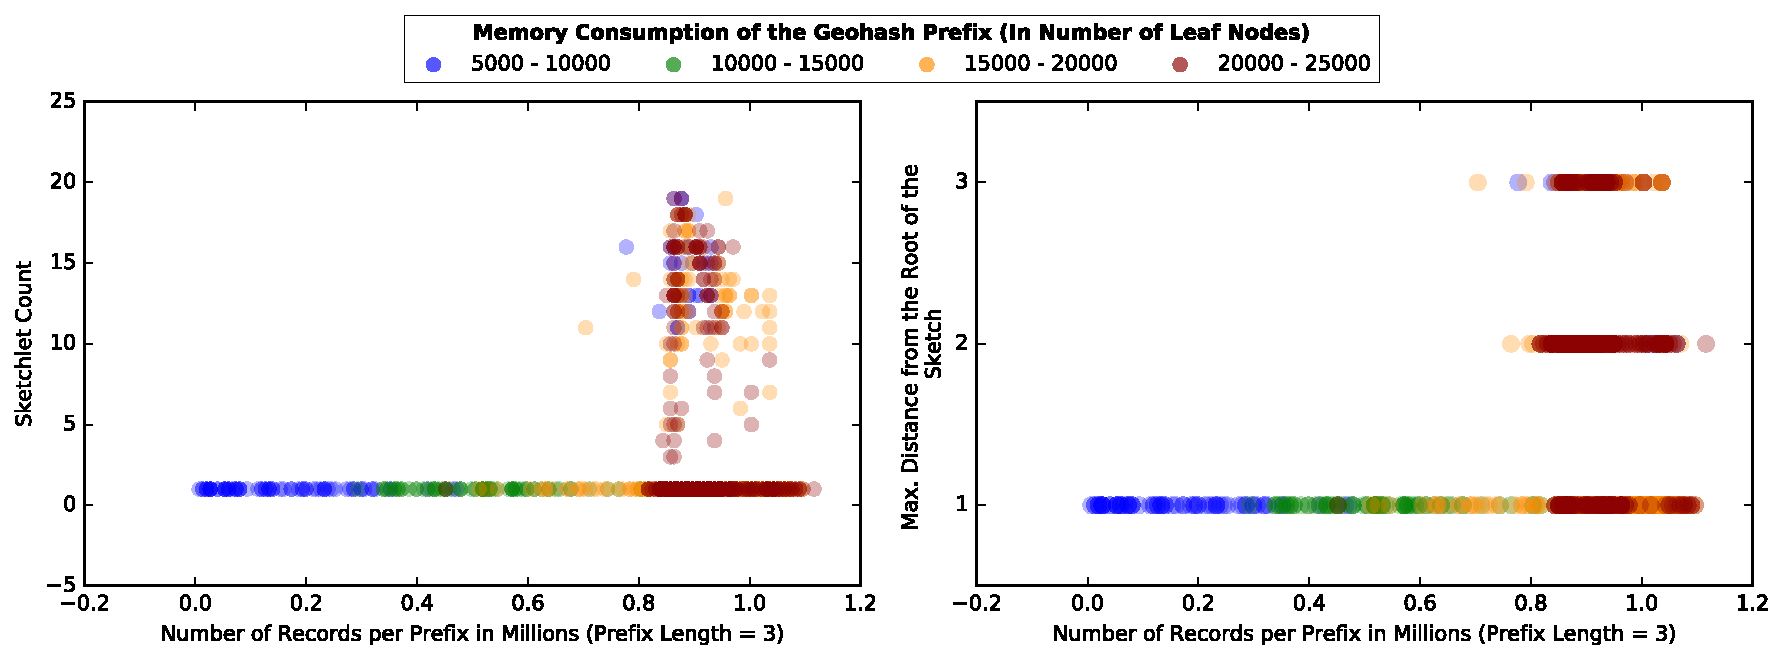
\includegraphics[width=\linewidth]{figures/scaleout_graph_analysis.pdf}}
    \caption{Analysis of a snapshot of the distributed sketch during data ingestion demonstrating the size and distribution of the information corresponding to different prefixes against the observed record count. If the information is dispersed over multiple sketchlets, it is likely to be a prefix with higher number of records and/or a wide range of observed values.}
    \label{fig:scaleout-graph-analysis}
\end{figure*}
%
\subsection{Analyzing a Snapshot of the Distributed Sketch}
Figure~\ref{fig:scaleout-graph-analysis} visualizes a snapshot of the distributed sketch which demonstrates the organization of sketchlets at runtime as described in \S\ref{sec:methodology}. 
This represents the state of the system after consuming the complete 2014 NOAA dataset, resulting in 48 sketchlets. 
The figure shows the distribution and size of the information maintained across sketchlets for each geohash prefix of 3 characters against the number of records processed for that particular prefix.
The memory requirement for a particular geohash prefix depends on the number of records as well as the range of the observed values for different features.
The space requirement is measured by the number of leaf nodes in the corresponding sketchlets.
For the majority of the prefixes, the space requirement increases with the number of records processed.
If the data for a particular prefix is distributed across multiple sketchlets, then it is more likely to be a prefix with a high number of records as shown in the first subplot.
In such cases, some of these sketchlets are created in multiple scale-out iterations, which results in a higher distance from the root of the prefix tree. This is depicted in the second subfigure of Figure~\ref{fig:scaleout-graph-analysis}.
A few prefixes with a high number of records can be observed with low memory consumption, and are distributed across multiple sketchlets; their observations span a smaller range, hence they require less memory but were chosen for scaling out operations due to their high message rates. 

\subsection{Dynamic Scaling: Responding to Variable Load}
%
\begin{figure}[b!]
    \centerline{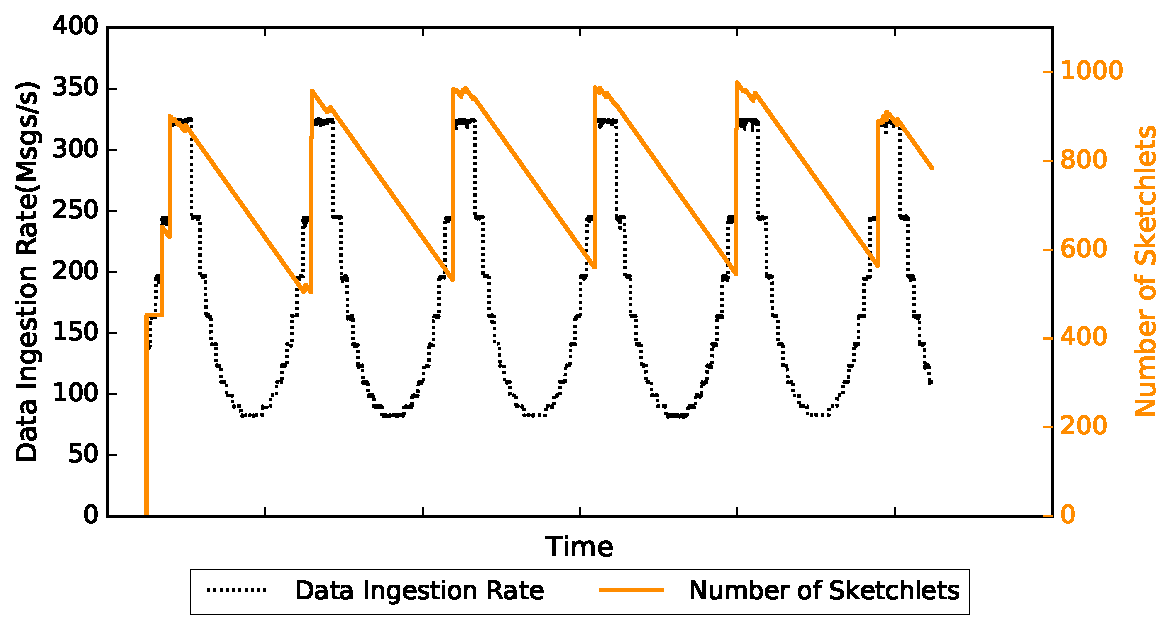
\includegraphics[width=3.5in]{figures/dyn-scaling.pdf}}
    \caption{Responding to variable load using dynamic scaling.}
    \label{fig:dyn-scaling}
\end{figure}
%
We evaluated how \textsc{Synopsis} dynamically scales when the data ingestion rate is varied.
The data ingestion rate was varied over time such that the peak data ingestion rate is higher than the highest possible cumulative throughput to create a backlog at sketchlets.
We augmented the sketch update code with additional operations to match the relatively low ingestion rates used for better control.
We used the number of sketchlets within the system to quantify the scaling activities.
If the system scales out, more sketchlets will be created as a result of targeted load migration.
We started with a single sketchlet and allowed the system to dynamically scale.
As can be observed in Figure~\ref{fig:dyn-scaling}, the number of sketchlets varies with the ingestion rate.
Since we allow aggressive scale-out, rapid scaling out is observed during high data ingestion rates whereas scaling in takes place gradually with one subregion (one sketchlet) at a time.

\subsection{Query Evaluation Performance}
\begin{figure*}
    \centerline{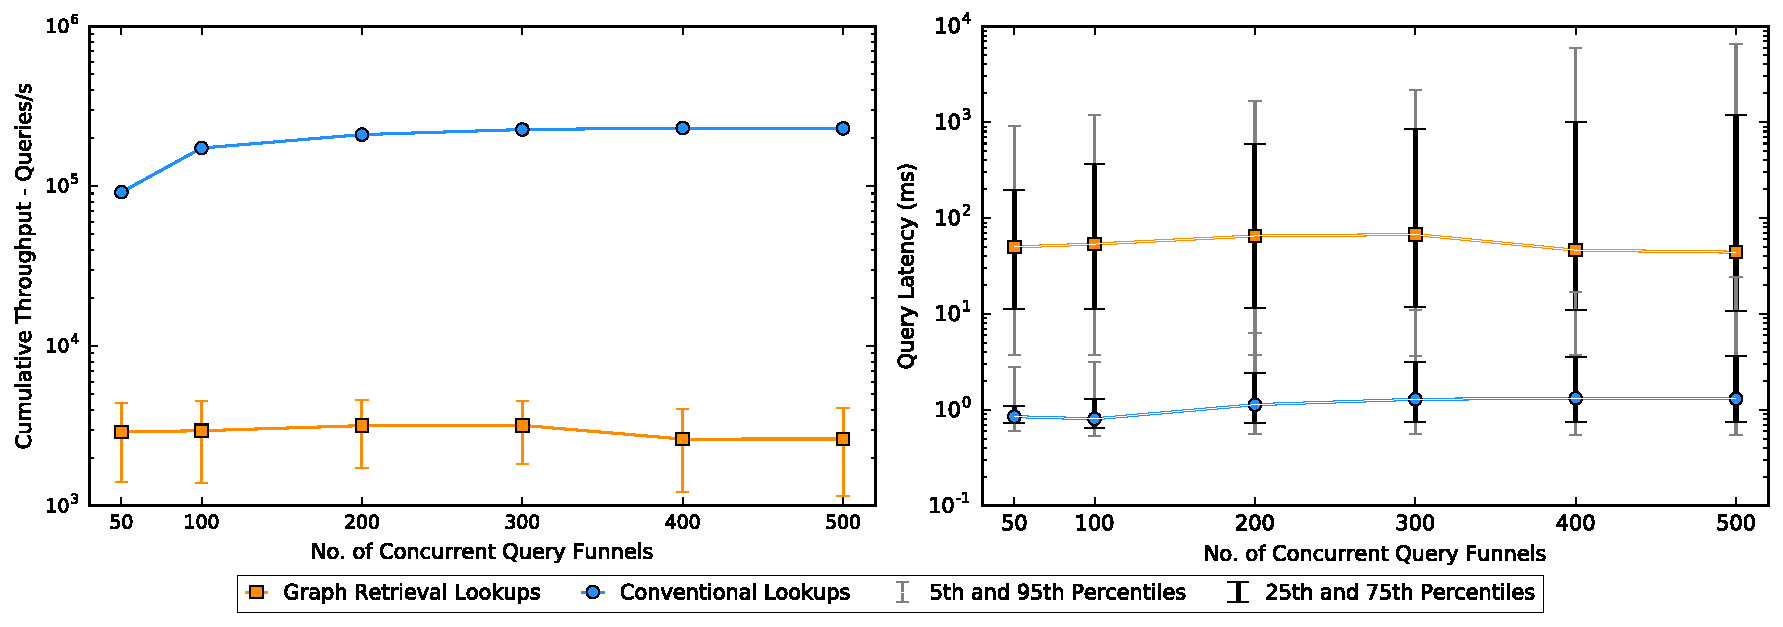
\includegraphics[width=\linewidth]{figures/query_benchmark_both.pdf}}
    \caption{Distributed query evaluation performance --- cumulative throughput and latency in a 40-node \textsc{Synopsis} cluster.}
    \label{fig:dist-query}
\end{figure*}
To evaluate distributed query performance, we executed representative workloads based on observed access patterns over our test dataset across a variety of sketchlet sizes. These queries were categorized as conventional lookups and tree retrievals.  Figure~\ref{fig:dist-query} depicts the end-to-end efficiency of the query evaluations over the distributed sketch.
Cumulative query throughput and latencies were measured with varying numbers of \emph{concurrent query funnels}.
A query funnel continuously generates and dispatches representative queries at the maximum possible rate to stress test the system and saturate its capacity. For example, a query could request summary statistics or feature relationships when the temperature is 20--30$^{\circ}$, humidity is above 80\%, and the wind speed is 16 km/h.
These queries fluctuated in both the ranges of values and spatial scope, resulting in high variability in the number of sketchlets required to resolve the query as well as the depth and breadth of the tree traversals.

Next we evaluated the query speedup gained by maintaining an in-memory sketch of the data compared to a traditional ETL pipeline.
We extracted the timestamp, location information (as a geohash), temperature, surface visibility, humidity and precipitation in the southeast United States during the months of May--August, 2011--2014 and loaded them into Spark as a DataFrame which was then queried using Spark SQL.
Given that the underlying RDD of the DataFrame cannot be shared between multiple Spark applications, we used a multi-threaded driver to issue concurrent queries.
Similarly, \textsc{Synopsis} was evaluated using a multi-threaded query funnel.
In order to minimize the data transfer between the Spark cluster and the driver, a \texttt{count} action was performed on the results of the SQL query and its result was retrieved at the client.
For \textsc{Synopsis}, we performed equivalent tree retrieval queries where sections of the distributed sketch is serialized and sent back to the query funnel.
End-to-end latencies of the queries were recorded for different concurrency levels.
Spark was evaluated under two different settings: caching enabled and disabled for the Dataframe.
The results of this evaluation is depicted in Figure~\ref{fig:spark-sql-query}.
%
\begin{figure}[b!]
    \centerline{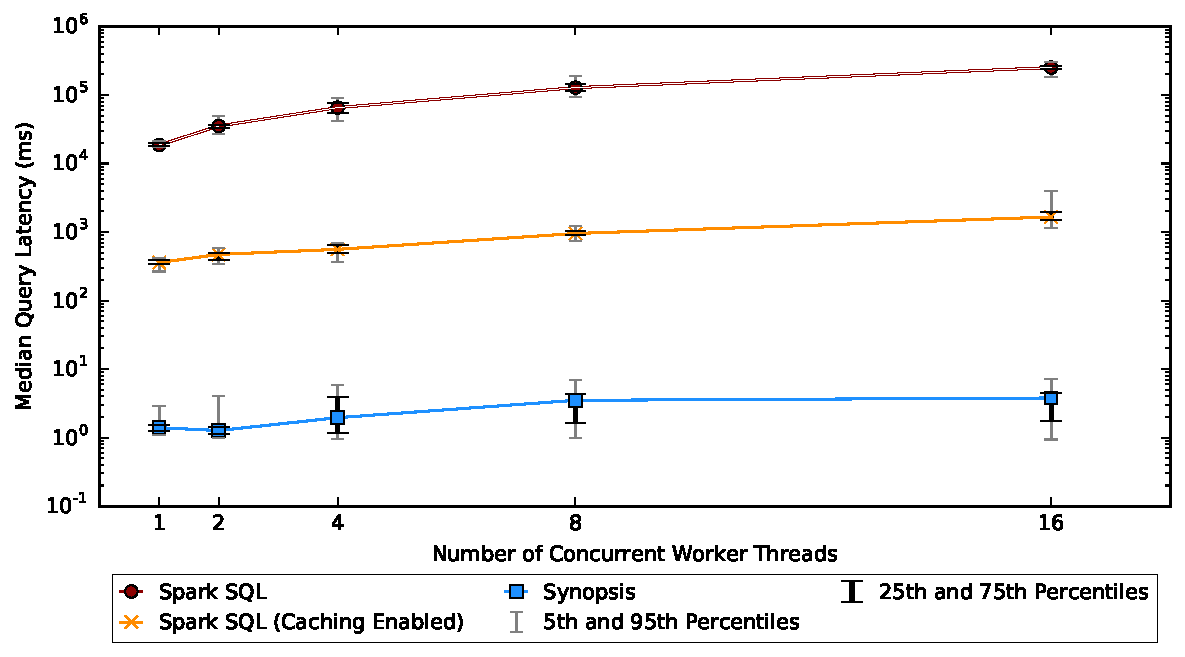
\includegraphics[width=\linewidth]{figures/spark-sql-query-complete.pdf}}
    \caption{Contrasting \textsc{Synopsis} query performance with an ETL system built with Spark SQL.}
    \label{fig:spark-sql-query}
\end{figure}
%
When caching is enabled, the Dataframe will be pinned in memory once materialized for the first time reducing the subsequent access times. Caching the entire Dataframe in memory may not be feasible in most real world spatiotemporal analytical tasks where the size of the dataset exceeds the available memory capacity of the cluster.
The end-to-end latency of the \textsc{Synopsis} queries is significantly less despite the larger size of the query results (section of the sketch for \textsc{Synopsis} vs the number of matching records for Spark SQL) transferred from the cluster to the query funnel.
Spark queries provides higher accuracy because queries are answered after scanning the entire dataset, but it requires more resources --- mainly memory and storage -- and incurs higher query latencies.
Resource requirements and query latencies with such ETL systems drastically increase with the number of features and geospatial and temporal scopes.
%
% Applicatons
%
\section{Applications}
\label{sec:applications}
Herein we profile the effectiveness of \textsc{Synopsis} as a surrogate for on-disk data in visualization and analytical settings.
\subsection{Visualization}
To demonstrate the potential applications of \textsc{Synopsis}, we created two visualizations. Our first visualization generated a climate chart by issuing statistical queries to retrieve high, low, and mean temperature values as well as precipitation information for a given spatial region. Climate charts are often used to provide a quick overview of the weather for a location; Figure~\ref{fig:climate} summarizes the temperature and precipitation in Snowmass Village, Colorado during 2014. While a standard approach for producing these visualizations over voluminous atmospheric data would likely involve several MapReduce computations, our sketchlets make all the necessary information readily available through queries, avoiding distributed computations altogether. Furthermore, retrieving the data for this evaluation consumed considerably less time (1.5 ms) than rendering the image on the client side (127.1 ms).
%
\begin{figure}[b]
    \centerline{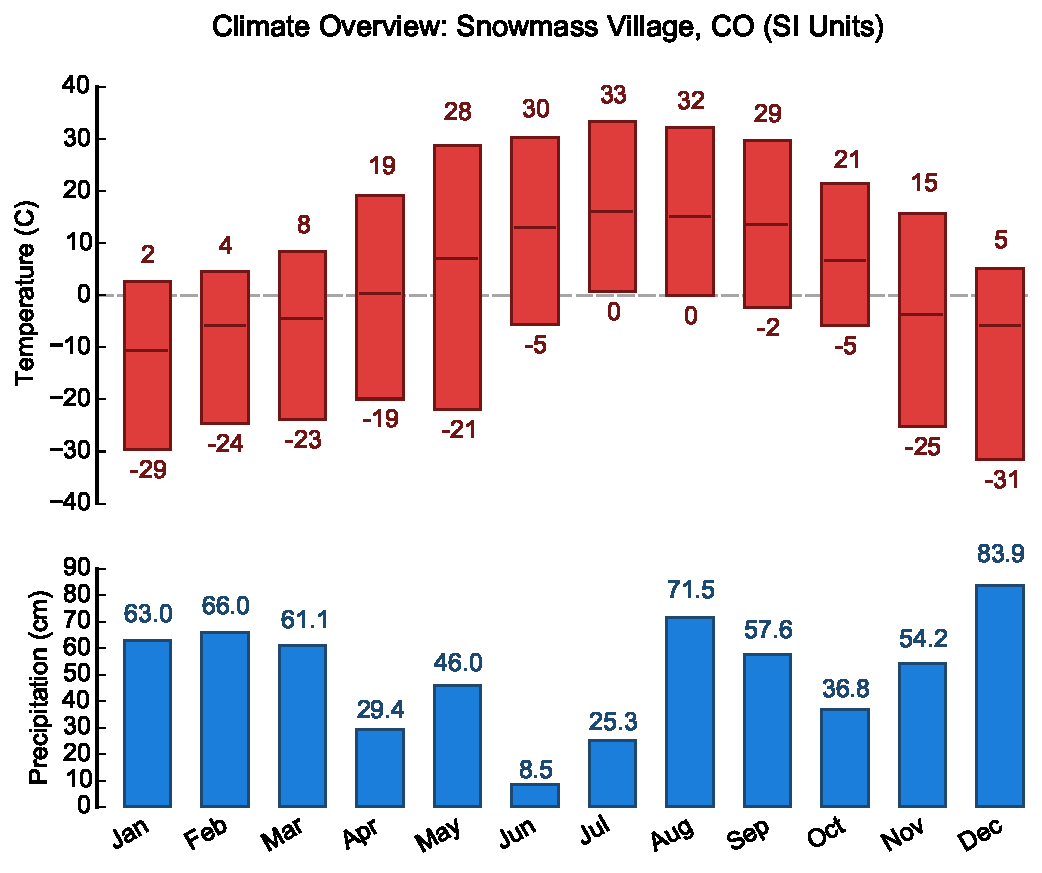
\includegraphics[width=0.85\linewidth]{figures/climate-snowmass.pdf}}
    \caption{A climate chart generated using a statistical query.}
    \label{fig:climate}
\end{figure}

Our second visualization issued queries to retrieve cloud cover information for the entirety of North America. To reduce processing load on the client side, we specified minimum visibility thresholds to eliminate data points that would not be visible in the final output figure. After retrieving this information, we executed a second query that located all areas that exhibited high correlations between cloud cover and precipitation. Figure~\ref{fig:global-contour} illustrates the results of this process for data in July of 2014; cloud cover is represented by white contours with varying opacity, while blue contours describe the correlation between cloud cover and precipitation (darker blues, such as those seen in the top-center of the globe, represent a stronger correlation). Due to the large scope of this visualization (retrieving all data points for a given month across all spatial regions), retrieval took approximately 2.82 seconds, with graphics rendering consuming an additional 1.51 seconds at the client application.
%
\begin{figure}[b]
    \centerline{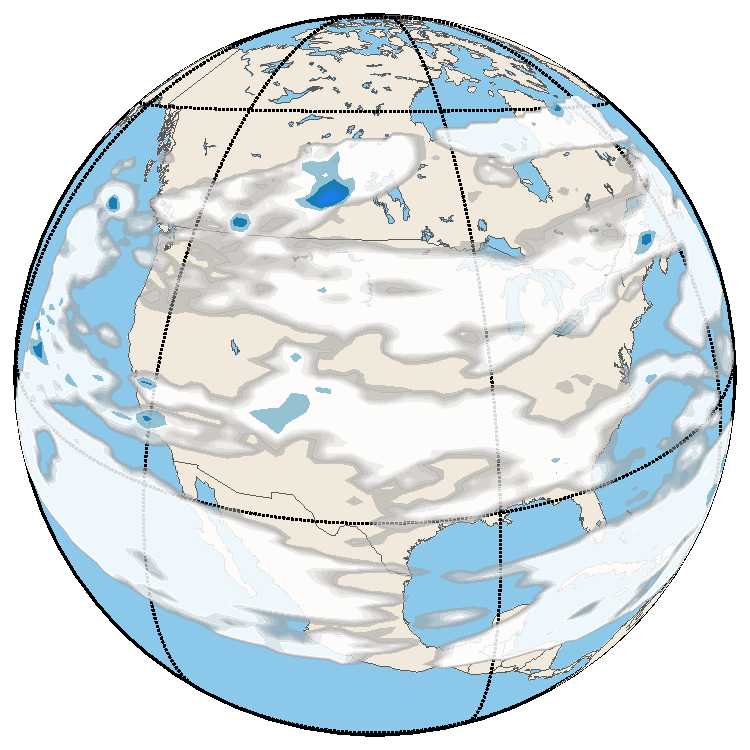
\includegraphics[width=2.2in]{figures/globe.pdf}}
    \caption{Global contour visualization showing cloud cover (white contours) and the correlation with precipitation (blue contours) in July of 2014 across North America.}
    \label{fig:global-contour}
\end{figure}

\subsection{Use with Analytic Engines}
Synthetic data queries in \textsc{Synopsis} can be used to generate representative datasets that require less space while still providing high accuracy.  
Such datasets can be used efficiently with analytic engines such as Apache Spark \cite{zaharia2010spark} and TensorFlow \cite{tensorflow}.  
We used Spark to train regression models based on the Random Forest ensemble method to predict temperatures (in Kelvin) using surface visibility, humidity and precipitation in the southeast United States during the months of May--August, 2011--2014.
These models were generated using the original full-resolution data as well as synthetic data sets that were sized at 10\%, 20\%, and 100\% of the original data.
For another point of comparison, we also generated datasets using 10\% and 20\% samples of the original data.
The accuracy of these models was measured using a test dataset extracted from actual observations (30\% of the overall dataset size).
All five datasets were staged on HDFS and loaded into Spark to train the models.

We evaluated our approach based on the on-disk and in-memory storage requirements, data loading time, training time and the accuracy of the model.
Our observations are summarized in Table~\ref{tab:spark-rf}; overall, the accuracy of the synthetic data models is comparable to that of the actual data, while requiring less space, training, and loading times;
for instance, our 10\% synthetic dataset produces a model with similar accuracy while incurring 54\% less training time and reducing space requirements by 90\%. Additionally, based on the number of RDD partitions used, the smaller synthetic datasets require substantially less computing resources.  It is worth noting that these particular models do not appear to benefit from a larger set of training samples, and could potentially begin to exhibit over-fitting if trained on more data.
We believe signs of this are demonstrated by the 100\% synthetic dataset, where fidelity limits of the sketch result in training data points that slightly decrease the expressiveness of the model. \vspace{-1em}
%
\begin{table*}[ht!]
    \renewcommand{\arraystretch}{1.2}
    \caption{Comparing Random Forest based regression models generated by Spark MLlib using synthetic vs. real data \vspace{-1em}}
    \label{tab:spark-rf}
    \begin{center}
        \begin{tabularx}{\textwidth}{|X|c|c|c|c|c|c|c|c|}
            \hline
            \multirow{2}{*}{Dataset} & \multirow{2}{*}{Size (GB)} & \multirow{2}{*}{RDD Partitions} & \multicolumn{2}{c|}{\cellcolor[gray]{0.7}Data Loading Time (s)} &\multicolumn{2}{c|}{\cellcolor[gray]{0.7}Model Training Time (s)} & \multicolumn{2}{c|}{\cellcolor[gray]{0.7}Accuracy - RMSE (K)}\\
            \cline{4-9}
             & & & \cellcolor[gray]{0.9}Mean & \cellcolor[gray]{0.9}Std. Dev.  &  \cellcolor[gray]{0.9}Mean & \cellcolor[gray]{0.9}Std. Dev. &  \cellcolor[gray]{0.9}Mean & \cellcolor[gray]{0.9}Std. Dev. \\
            \hline
            Original & 25.350 & 208 & 28.035 & 2.249 & 506.493 & 9.500 & 5.981 & 0.027 \\
            \hline
            Original - 10\% Sample & 2.535 & 21 & 5.136 & 0.909 & 205.627 & 5.798 & 5.960  & 0.049 \\
            \hline
            Original - 20\% Sample & 5.069 & 41 & 6.102 & 1.607 & 216.857 & 7.994 & 5.994 & 0.026 \\
            \hline
            Synthetic - 10\% & 2.549 & 21 & 5.097 & 0.912 & 231.221 & 13.459 & 5.951 & 0.027 \\
            \hline
            Synthetic - 20\% & 5.098 & 41 & 6.208 & 0.637 & 235.018 & 16.148 & 5.981 & 0.051 \\
            \hline
            Synthetic - 100\% & 25.066 & 207 & 25.670 & 2.947 & 454.964 & 16.446 & 6.192 & 0.076 \\
            \hline
        \end{tabularx}
    \end{center}
    \vspace{-1em}
\end{table*}
%
% Related Work
%
\section{Related Work}
\label{sec:related}
Tao et al.~\cite{tao2004spatio} answers distinct sum and count queries over spatiotemporal data with a sketch index similar to an aRB-tree~\cite{papadias2002indexing} where spatial indexing is implemented is using an R-tree and temporal indexing is implemented as a B-tree.  At the leaf nodes of the B-tree, a sketch that follows the Flajolet-Martin algorithm~\cite{flajolet1985probabilistic} is used to capture an approximate view of the observations.
This approach significantly reduces the space requirements for answering distinct sum/count queries on spatiotemporal data and provides efficient query evaluations due to its ability to prune portions of the search space.
\textsc{Synopsis} differs in its ability to capture multiple features and their interactions, which facilitates a broader set of queries.

Data~Cubes~\cite{gray1996data,harinarayan1996implementing,mumick1997maintenance,ho1997range} are a data structure for Online Analytical Processing that provide multidimensional query and summarization functionality. These structures generalize several operators provided by relational databases by projecting two-dimensional relational tables to N-dimensional cubes (also known as \emph{hypercubes} when $N > 3$). Variable resolution in Data Cubes is managed by the \emph{drill down/drill up} operators, and \emph{slices} or entire cubes can be summarized through the \emph{roll up} operator. While Data Cubes provide many of the same features supported by \textsc{Synopsis}, they are primarily intended for single-host offline or batch processing systems due to their compute- and data-intensive updates. In fact, many production deployments separate transaction processing and analytical processing systems, with updates pushed to the Data Cubes periodically. 

%CHAOS~\cite{gupta2009chaos} builds on Data Cubes in a single-host streaming environment by pushing updates to its \emph{Computational Cubes} more frequently. To make dimensionality and storage requirements manageable, Computational Cubes only index summaries of incoming data that are generated during a preprocessing step. However, full-resolution data is still made available through continuous queries that act on variable-length sliding windows.  CHAOS builds its summaries using a wavelet-based approach, which tend to be highly problem-specific. Additionally, updates to the cube are still generated and published periodically rather than immediately as data is assimilated. 

Galileo~\cite{malensek2016analytic,malensek2015fast} is a distributed hash table that supports the storage and retrieval of multidimensional data. Given the overlap in problem domain, Galileo is faced with several of the same challenges as \textsc{Synopsis}. However, the avenues for overcoming these issues diverge significantly due to differences in storage philosophy: \textsc{Synopsis} maintains its dataset completely in main memory, avoiding the orders-of-magnitude disparity in I/O throughput associated with secondary storage systems. This makes \textsc{Synopsis} highly agile, allowing on-demand scaling to rapidly respond to changes in incoming load. Additionally, this constraint influenced the trade-off space involved when designing our algorithms, making careful and efficient memory management a priority while striving for high accuracy.

Simba (Spatial In-Memory Big data Analytics)~\cite{xiesimba} extends Spark SQL~\cite{armbrust2015spark} to support spatial operations in SQL as well as DataFrames. It relies on data being stored in Spark~\cite{zaharia2010spark}. Despite its higher accuracy, it is not scalable for geospatial streams in the long term due to high storage requirements. In \textsc{Synopsis}, spatial queries can be executed with a reasonable accuracy without having to store the streaming data as-is.

Dynamic scaling and elasticity in stream processing systems has been studied thoroughly \cite{heinze2014auto, gulisano2012streamcloud, castro2013integrating, loesing2012stormy, heinze2013elastic, schneider2009elastic}.
%Heinze et al.~\cite{heinze2014auto} explores different dynamic scaling schemes including threshold-based rules and reinforcement learning using the FUGU~\cite{heinze2013elastic} stream processing engine.
%Based on these schemes, the operators are continuously migrated between hosts in a FUGU cluster in order to optimize the resource utilization and to maintain low latency.
%The approach is quite different from \textsc{Synopsis}, as we perform a targeted load migration where the workload of a computation is dynamically adjusted instead of entirely moving it to a host with a higher or lower capacity than the current host.
%Further, we do not interrupt the data flow through \textsc{Synopsis} when dynamic scaling activities are in progress, whereas in FUGU the predecessor operator is temporarily paused until operator migration completes.
StreamCloud~\cite{gulisano2012streamcloud} relies on a global threshold-based scheme to implement elasticity where a query is partitioned into sub-queries which run on separate clusters.
It relies on a centralized component, the Elastic Manager, to initiate the elastic reconfiguration protocol, whereas in \textsc{Synopsis} each node independently initiates the dynamic scaling protocol.
This difference is mainly due to different optimization objectives of the two systems; StreamCloud tries to optimize the average CPU usage per cluster while \textsc{Synopsis} attempts to maintain stability at each node.
The state recreation protocol of StreamCloud is conceptually similar to our state transfer protocol, except that tuples are buffered at the new location until the state transfer is complete, whereas in \textsc{Synopsis} the new sketchlet immediately starts building the state which is later merged with the state (transferred asynchronously) from the parent sketchlet.

Gedik et al.~\cite{schneider2009elastic} also uses a threshold-based local scheme similar to \textsc{Synopsis}. Additionally, this approach keeps track of the past performance achieved at different operating conditions in order to avoid oscillations in scaling activities.
The use of consistent hashing at the splitters (similar to geohash based stream partitioning in \textsc{Synopsis}) achieves both load balancing and monotonicity (elastic scaling does not move states between nodes that are present before and after the scaling activity).
Similarly, our geohash-based partitioner together with control algorithms in \textsc{Synopsis} balance the workload by alleviating hotspots and sketchlets with lower resource utilization.
Our state migration scheme doesn't require migrating states between sketchlets that do not participate in the scaling activity, unlike with a reconfiguration of a regular hash-based partitioner.
Unlike in \textsc{Synopsis}, in their implementation, the stream data flow is paused until state migration is complete using vertical and horizontal barriers.
Finally, \textsc{Synopsis}' scaling schemes are placement-aware, meaning certain nodes are preferred when performing scaling with the objective of reducing the span of the distributed sketch.
%
% Conclusion
%
\vspace{-1em}
\section{Conclusions and Future Work}
\label{sec:conclusions}
\textsc{Synopsis}, our framework for constructing a distributed sketch over spatiotemporal streams, is able to (1) maintain a compact representation of the observational space, (2) support dynamic scaling to preserve responsiveness and avoid overprovisioning, and (3) explore the observational space with a rich set of queries. Our methodology for achieving this is broadly applicable to other stream processing systems and our empirical benchmarks demonstrate the suitability of our approach.

We achieve compactness in our sketchlet instances by dynamically managing the number of vertices in the SIFT hierarchy as well as the range each vertex is responsible for. We also maintain summary statistics and metadata within these vertices to track the distribution/dispersion of feature values and their frequencies. As a result, \textsc{Synopsis} is able to represent datasets using substantially less memory (\textbf{RQ-1}). Given variability in the rates and volumes of data arrivals from different geolocations, our scaling mechanism avoids overprovisioning and alleviates situations where sketch updates cannot keep pace with data arrival rates. Memory pressure is also taken into account during replica creation as well as when scaling in and out (\textbf{RQ-2}). During evaluations, only the sketchlets that hold portions of the observational space implicitly or explicitly targeted by the query are involved, ensuring high throughput. We support several high-level query operations allowing users to locate and manipulate data efficiently (\textbf{RQ-3}).

Our future work will target support for \textsc{Synopsis} to be used as input for long-running computations. Such jobs would execute periodically on a varying number of machines and could target the entire observational space or only the most recently-assimilated records. We also plan to implement continuous queries that can autonomously evolve with the feature space.
\vspace{1em}\\
%
% Acknowledgement
%
\textbf{Acknowledgements:}
This research has been \hl{supported by funding from the US Deptartment of Homeland Security [D15PC00279]}; the US National Science Foundation [ACI-1553685, CNS-1253908]; and a Monfort Professorship.
% ensure same length columns on last page (might need two sub-sequent latex runs)
% \balance

\bibliographystyle{IEEEtran}
\bibliography{references}
\vspace*{-3.7\baselineskip}
\begin{IEEEbiography}[{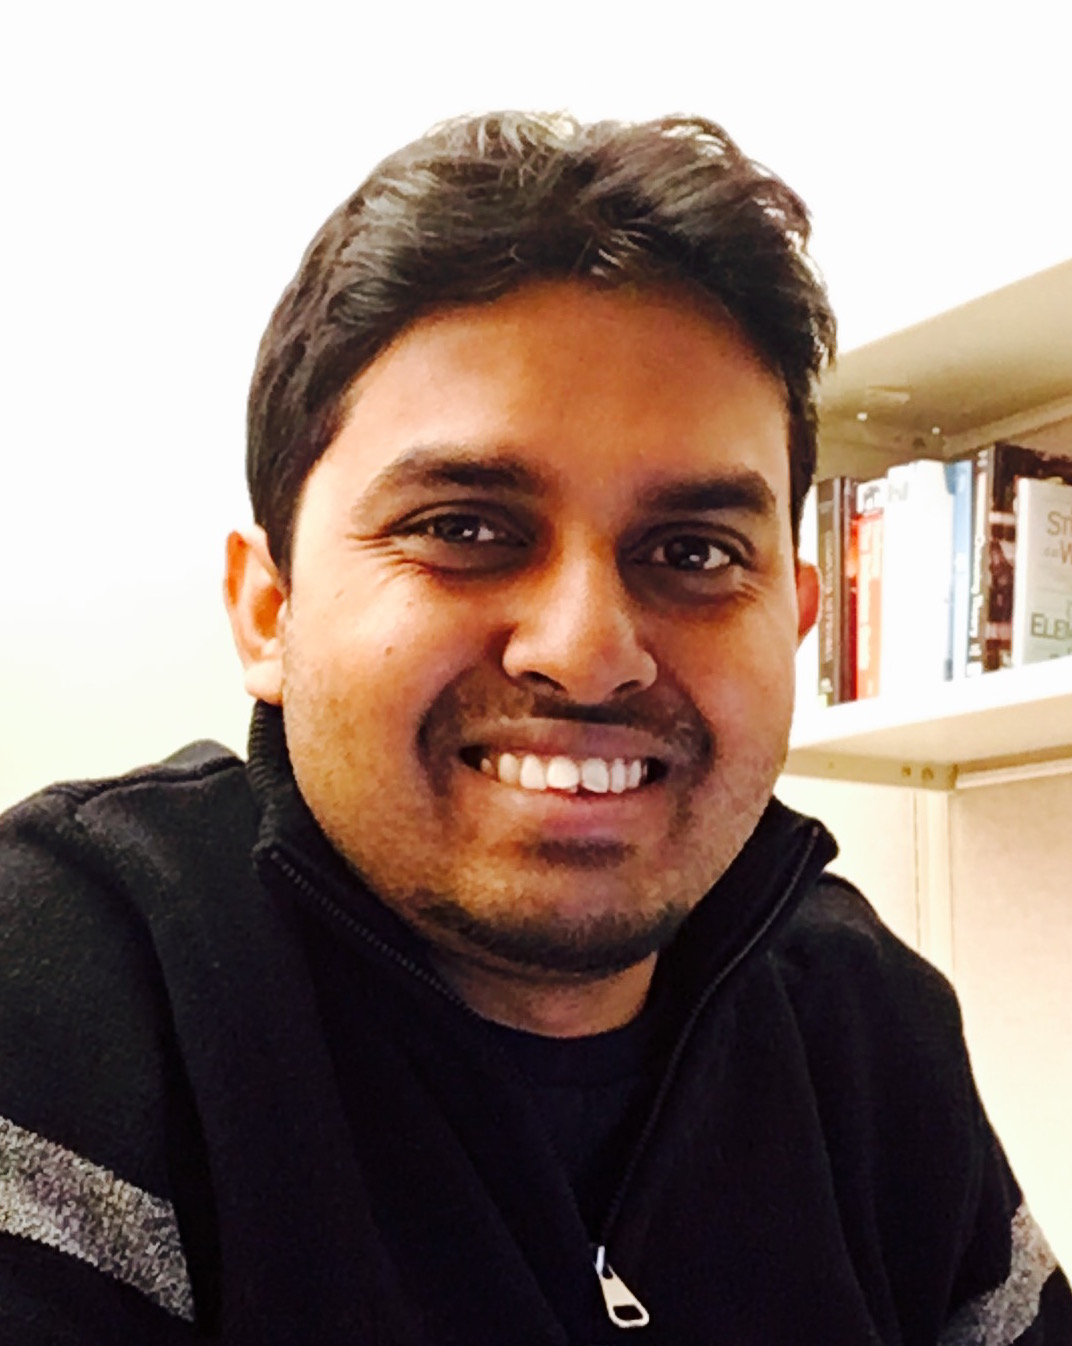
\includegraphics[width=1in,height=1.2in, clip,keepaspectratio]{./bio/thilina.jpg}}]{Thilina Buddhika} is a Ph.D. candidate in the Computer Science department at Colorado State University.  His research interests are in the area of real time, high throughput stream processing specifically targeted to environments such as Internet of Things (IoT) and health care applications. Email: thilinab@cs.colostate.edu
\end{IEEEbiography}
\vspace{-1.60cm}
\begin{IEEEbiography}[{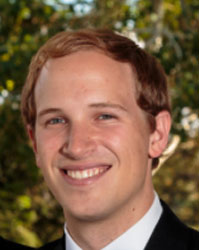
\includegraphics[width=1in,height=1.2in,clip,keepaspectratio]{./bio/matthew.jpg}}]{Matthew Malensek} \hl{received his Ph.D. from the Department of Computer Science at Colorado State University.} His research involves the design and implementation of large-scale distributed systems, data-intensive computing, and cloud computing. Email: malensek@cs.colostate.edu
\end{IEEEbiography}
%
\vspace{-1.60cm}
\begin{IEEEbiography}[{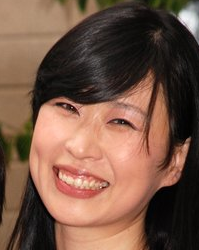
\includegraphics[width=1in,height=1.2in,clip,keepaspectratio]{./bio/sangmi.jpg}}]{Sangmi Lee Pallickara} is an Associate Professor in the Department of Computer Science at Colorado State University. She received her Masters and Ph.D. degrees in Computer Science from Syracuse University and Florida State University, respectively. Her research interests are in the area of large-scale scientific data management. She is a recipient of the NSF CAREER award. Email: sangmi@cs.colostate.edu
\end{IEEEbiography}
%
\vspace{-1.56cm}
\begin{IEEEbiography}[{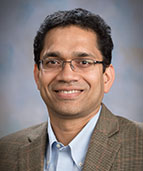
\includegraphics[width=1in,height=1.2in,clip,keepaspectratio]{./bio/shrideep.jpg}}]{Shrideep Pallickara} is an Associate Professor in the Department of Computer Science and a Monfort Professor at Colorado State University. His research interests are in the area of large-scale distributed systems. He received his Masters and Ph.D. degrees from Syracuse University. He is a recipient of an NSF CAREER award. Email: shrideep@cs.colostate.edu
\enlargethispage{0.7cm}
\end{IEEEbiography}
\end{document}
